%% 
%% Analysis 1&2 BSc, ETH
%%
%% (C) 2012 Gregor Wegberg
%%
%% Contributors:
%%   - Leo Büttiker
%%   - Benjamin Steger
%% 
%% License: Creative Commons Attribution-Share Alike 3.0 Unported
%% http://creativecommons.org/licenses/by-sa/3.0/
%% 


\documentclass[a4paper,titlepage,twocolumn]{article}
\usepackage[ngerman]{babel}

%%
%% 
%% (C) 2011 Gregor Wegberg
%%
%% Based on work of Stefan Heule, Licensed as Creative Commons Attribution-Share Alike 3.0 Unported
%% 
%% License: Creative Commons Attribution-Share Alike 3.0 Unported
%% http://creativecommons.org/licenses/by-sa/3.0/
%% 

%% The following lines need to be included in the main tex file
%\documentclass[portrait,a4paper,titlepage]{article}
%%%
%% 
%% (C) 2011 Gregor Wegberg
%%
%% Based on work of Stefan Heule, Licensed as Creative Commons Attribution-Share Alike 3.0 Unported
%% 
%% License: Creative Commons Attribution-Share Alike 3.0 Unported
%% http://creativecommons.org/licenses/by-sa/3.0/
%% 

%% The following lines need to be included in the main tex file
%\documentclass[portrait,a4paper,titlepage]{article}
%%%
%% 
%% (C) 2011 Gregor Wegberg
%%
%% Based on work of Stefan Heule, Licensed as Creative Commons Attribution-Share Alike 3.0 Unported
%% 
%% License: Creative Commons Attribution-Share Alike 3.0 Unported
%% http://creativecommons.org/licenses/by-sa/3.0/
%% 

%% The following lines need to be included in the main tex file
%\documentclass[portrait,a4paper,titlepage]{article}
%\input{standard-definitions.tex}

\usepackage[utf8]{inputenc}
\usepackage{fontenc}

\usepackage{color}
\usepackage{soul}
\usepackage{soulutf8}

% Stichwortverzeichnis
\usepackage{makeidx}
%\usepackage{idxlayout}

\usepackage{alltt}
\renewcommand{\ttdefault}{txtt}

\usepackage{amssymb,amsfonts,amsmath}
\usepackage[e]{esvect}

\usepackage{algorithmicx}

\usepackage[pdftex]{graphicx}
\usepackage{epstopdf}
\usepackage[svgnames]{xcolor}

\usepackage{cancel}

\usepackage{pgf,tikz}
\usetikzlibrary{arrows}

\usepackage{geometry}
\geometry{a4paper, left=20mm, right=20mm, top=25mm, bottom=20mm}

% Allows fancy stuff in the page header
\usepackage{fancyhdr}
\pagestyle{fancy}

% hyperref
\usepackage[colorlinks=false,pdfborder={0 0 0}]{hyperref}

% multirow and multicol
\usepackage{multirow}
\usepackage{multicol}
\columnsep24pt
\columnseprule0.1pt

% enumerate
\renewcommand\theenumi{\arabic{enumi}}
\renewcommand\labelenumi{\theenumi.}
\renewcommand\theenumii{\roman{enumii}}
\renewcommand\labelenumii{\theenumii)}

\usepackage{listings}
\lstset{
    floatplacement={tbp}
    basicstyle=\ttfamily\mdseries,
    identifierstyle=,
    stringstyle=\color{gray},
    numbers=left,
    numbersep=5pt,
    inputencoding=utf8,
    xleftmargin=8pt,
    xrightmargin=8pt,
    keywordstyle=[1]\bfseries,
    keywordstyle=[2]\bfseries,
    keywordstyle=[3]\bfseries,
    keywordstyle=[4]\bfseries,
    numberstyle=\tiny,
    stepnumber=1,
    breaklines=true,
    frame=lines,
    showstringspaces=false,
    tabsize=2,
    commentstyle=\color{gray},
    captionpos=b,
    float=float,
    language={Java}
}
\newcommand{\code}[1]{\lstinline{#1}}

% depth of section numbering
\setcounter{secnumdepth}{4}

%% Redefine the \paragraph command:
\makeatletter
\renewcommand\paragraph{\@startsection{paragraph}{4}{0mm}%
    {-\baselineskip}%
    {0.5\baselineskip}%
    {\normalfont\bfseries}%
}%
\makeatother

% parindent
\parindent0px
\parskip3pt

% redefine greek letters
\renewcommand{\phi}{\varphi}
\renewcommand{\epsilon}{\varepsilon}

% shortcuts in math mode
\newcommand{\bs}{\boldsymbol}
\newcommand{\mc}{\mathcal}
\newcommand{\norm}[1]{| \!\:\! | #1 | \!\:\! |}
\newcommand{\with}{\;|\;} % with in set notation
\newcommand{\ds}{\displaystyle}
\newcommand{\nop}[1]{}
\newcommand{\argmax}{\operatorname*{arg\;max}}
\newcommand{\argmin}{\operatorname*{arg\;min}}
\newcommand{\rmd}{\mathrm{d}} % for integrals
\newcommand{\ggT}{\operatorname*{ggT}}
\newcommand{\kgV}{\operatorname*{kgV}}
\newcommand{\id}{\operatorname{id}}
\newcommand{\grad}{\operatorname{grad}}
\newcommand{\rot}{\operatorname{rot}}

% number sets
\newcommand{\R}{\mathbb{R}}
\newcommand{\Z}{\mathbb{Z}}
\newcommand{\N}{\mathbb{N}}
\newcommand{\Q}{\mathbb{Q}}
\newcommand{\C}{\mathbb{C}}
\newcommand{\F}{\mathbb{F}}
\newcommand{\E}{\mathbb{E}}
\newcommand{\LL}{\mathcal{L}}
\newcommand{\powerset}{\mathcal P}

% probabilities
\newcommand{\Prob}[1]{\operatorname{Pr}\left[#1\right]}
\newcommand{\Ex}[1]{\mathbb{E}\left[#1\right]}

% todo
\newcommand{\todo}[1]{\sethlcolor{red}\hl{$\ggg$ \textbf{TODO} [#1]}\sethlcolor{yellow}}


% big-o notation
\newcommand{\bigO}[1]{\mc O\left(#1\right)}




\usepackage[utf8]{inputenc}
\usepackage{fontenc}

\usepackage{color}
\usepackage{soul}
\usepackage{soulutf8}

% Stichwortverzeichnis
\usepackage{makeidx}
%\usepackage{idxlayout}

\usepackage{alltt}
\renewcommand{\ttdefault}{txtt}

\usepackage{amssymb,amsfonts,amsmath}
\usepackage[e]{esvect}

\usepackage{algorithmicx}

\usepackage[pdftex]{graphicx}
\usepackage{epstopdf}
\usepackage[svgnames]{xcolor}

\usepackage{cancel}

\usepackage{pgf,tikz}
\usetikzlibrary{arrows}

\usepackage{geometry}
\geometry{a4paper, left=20mm, right=20mm, top=25mm, bottom=20mm}

% Allows fancy stuff in the page header
\usepackage{fancyhdr}
\pagestyle{fancy}

% hyperref
\usepackage[colorlinks=false,pdfborder={0 0 0}]{hyperref}

% multirow and multicol
\usepackage{multirow}
\usepackage{multicol}
\columnsep24pt
\columnseprule0.1pt

% enumerate
\renewcommand\theenumi{\arabic{enumi}}
\renewcommand\labelenumi{\theenumi.}
\renewcommand\theenumii{\roman{enumii}}
\renewcommand\labelenumii{\theenumii)}

\usepackage{listings}
\lstset{
    floatplacement={tbp}
    basicstyle=\ttfamily\mdseries,
    identifierstyle=,
    stringstyle=\color{gray},
    numbers=left,
    numbersep=5pt,
    inputencoding=utf8,
    xleftmargin=8pt,
    xrightmargin=8pt,
    keywordstyle=[1]\bfseries,
    keywordstyle=[2]\bfseries,
    keywordstyle=[3]\bfseries,
    keywordstyle=[4]\bfseries,
    numberstyle=\tiny,
    stepnumber=1,
    breaklines=true,
    frame=lines,
    showstringspaces=false,
    tabsize=2,
    commentstyle=\color{gray},
    captionpos=b,
    float=float,
    language={Java}
}
\newcommand{\code}[1]{\lstinline{#1}}

% depth of section numbering
\setcounter{secnumdepth}{4}

%% Redefine the \paragraph command:
\makeatletter
\renewcommand\paragraph{\@startsection{paragraph}{4}{0mm}%
    {-\baselineskip}%
    {0.5\baselineskip}%
    {\normalfont\bfseries}%
}%
\makeatother

% parindent
\parindent0px
\parskip3pt

% redefine greek letters
\renewcommand{\phi}{\varphi}
\renewcommand{\epsilon}{\varepsilon}

% shortcuts in math mode
\newcommand{\bs}{\boldsymbol}
\newcommand{\mc}{\mathcal}
\newcommand{\norm}[1]{| \!\:\! | #1 | \!\:\! |}
\newcommand{\with}{\;|\;} % with in set notation
\newcommand{\ds}{\displaystyle}
\newcommand{\nop}[1]{}
\newcommand{\argmax}{\operatorname*{arg\;max}}
\newcommand{\argmin}{\operatorname*{arg\;min}}
\newcommand{\rmd}{\mathrm{d}} % for integrals
\newcommand{\ggT}{\operatorname*{ggT}}
\newcommand{\kgV}{\operatorname*{kgV}}
\newcommand{\id}{\operatorname{id}}
\newcommand{\grad}{\operatorname{grad}}
\newcommand{\rot}{\operatorname{rot}}

% number sets
\newcommand{\R}{\mathbb{R}}
\newcommand{\Z}{\mathbb{Z}}
\newcommand{\N}{\mathbb{N}}
\newcommand{\Q}{\mathbb{Q}}
\newcommand{\C}{\mathbb{C}}
\newcommand{\F}{\mathbb{F}}
\newcommand{\E}{\mathbb{E}}
\newcommand{\LL}{\mathcal{L}}
\newcommand{\powerset}{\mathcal P}

% probabilities
\newcommand{\Prob}[1]{\operatorname{Pr}\left[#1\right]}
\newcommand{\Ex}[1]{\mathbb{E}\left[#1\right]}

% todo
\newcommand{\todo}[1]{\sethlcolor{red}\hl{$\ggg$ \textbf{TODO} [#1]}\sethlcolor{yellow}}


% big-o notation
\newcommand{\bigO}[1]{\mc O\left(#1\right)}




\usepackage[utf8]{inputenc}
\usepackage{fontenc}

\usepackage{color}
\usepackage{soul}
\usepackage{soulutf8}

% Stichwortverzeichnis
\usepackage{makeidx}
%\usepackage{idxlayout}

\usepackage{alltt}
\renewcommand{\ttdefault}{txtt}

\usepackage{amssymb,amsfonts,amsmath}
\usepackage[e]{esvect}

\usepackage{algorithmicx}

\usepackage[pdftex]{graphicx}
\usepackage{epstopdf}
\usepackage[svgnames]{xcolor}

\usepackage{cancel}

\usepackage{pgf,tikz}
\usetikzlibrary{arrows}

\usepackage{geometry}
\geometry{a4paper, left=20mm, right=20mm, top=25mm, bottom=20mm}

% Allows fancy stuff in the page header
\usepackage{fancyhdr}
\pagestyle{fancy}

% hyperref
\usepackage[colorlinks=false,pdfborder={0 0 0}]{hyperref}

% multirow and multicol
\usepackage{multirow}
\usepackage{multicol}
\columnsep24pt
\columnseprule0.1pt

% enumerate
\renewcommand\theenumi{\arabic{enumi}}
\renewcommand\labelenumi{\theenumi.}
\renewcommand\theenumii{\roman{enumii}}
\renewcommand\labelenumii{\theenumii)}

\usepackage{listings}
\lstset{
    floatplacement={tbp}
    basicstyle=\ttfamily\mdseries,
    identifierstyle=,
    stringstyle=\color{gray},
    numbers=left,
    numbersep=5pt,
    inputencoding=utf8,
    xleftmargin=8pt,
    xrightmargin=8pt,
    keywordstyle=[1]\bfseries,
    keywordstyle=[2]\bfseries,
    keywordstyle=[3]\bfseries,
    keywordstyle=[4]\bfseries,
    numberstyle=\tiny,
    stepnumber=1,
    breaklines=true,
    frame=lines,
    showstringspaces=false,
    tabsize=2,
    commentstyle=\color{gray},
    captionpos=b,
    float=float,
    language={Java}
}
\newcommand{\code}[1]{\lstinline{#1}}

% depth of section numbering
\setcounter{secnumdepth}{4}

%% Redefine the \paragraph command:
\makeatletter
\renewcommand\paragraph{\@startsection{paragraph}{4}{0mm}%
    {-\baselineskip}%
    {0.5\baselineskip}%
    {\normalfont\bfseries}%
}%
\makeatother

% parindent
\parindent0px
\parskip3pt

% redefine greek letters
\renewcommand{\phi}{\varphi}
\renewcommand{\epsilon}{\varepsilon}

% shortcuts in math mode
\newcommand{\bs}{\boldsymbol}
\newcommand{\mc}{\mathcal}
\newcommand{\norm}[1]{| \!\:\! | #1 | \!\:\! |}
\newcommand{\with}{\;|\;} % with in set notation
\newcommand{\ds}{\displaystyle}
\newcommand{\nop}[1]{}
\newcommand{\argmax}{\operatorname*{arg\;max}}
\newcommand{\argmin}{\operatorname*{arg\;min}}
\newcommand{\rmd}{\mathrm{d}} % for integrals
\newcommand{\ggT}{\operatorname*{ggT}}
\newcommand{\kgV}{\operatorname*{kgV}}
\newcommand{\id}{\operatorname{id}}
\newcommand{\grad}{\operatorname{grad}}
\newcommand{\rot}{\operatorname{rot}}

% number sets
\newcommand{\R}{\mathbb{R}}
\newcommand{\Z}{\mathbb{Z}}
\newcommand{\N}{\mathbb{N}}
\newcommand{\Q}{\mathbb{Q}}
\newcommand{\C}{\mathbb{C}}
\newcommand{\F}{\mathbb{F}}
\newcommand{\E}{\mathbb{E}}
\newcommand{\LL}{\mathcal{L}}
\newcommand{\powerset}{\mathcal P}

% probabilities
\newcommand{\Prob}[1]{\operatorname{Pr}\left[#1\right]}
\newcommand{\Ex}[1]{\mathbb{E}\left[#1\right]}

% todo
\newcommand{\todo}[1]{\sethlcolor{red}\hl{$\ggg$ \textbf{TODO} [#1]}\sethlcolor{yellow}}


% big-o notation
\newcommand{\bigO}[1]{\mc O\left(#1\right)}



\usepackage{geometry}
\usepackage{amsthm}
\usepackage{enumitem}

\setlist{nolistsep}

\geometry{top=1cm, headsep=0pt,headheight=0.5cm, % top part
bottom=1cm, footskip=0.5cm, % bottom part
left=0.4cm,right=0.4cm} % left / right part

% fancy header
\renewcommand{\footrulewidth}{0pt}
\renewcommand{\headrulewidth}{0pt}
\renewcommand{\headwidth}{\textwidth}

\tabcolsep=0.1cm

% Redefine section commands to use less space
\makeatletter
\renewcommand{\section}{\@startsection{section}{1}{0mm}%
                                {-1ex plus -.5ex minus -.2ex}%
                                {0.5ex plus .2ex}%x
                                {\normalfont\large\bfseries}}
\renewcommand{\subsection}{\@startsection{subsection}{2}{0mm}%
                                {-1explus -.5ex minus -.2ex}%
                                {0.5ex plus .2ex}%
                                {\normalfont\normalsize\bfseries}}
\renewcommand{\subsubsection}{\@startsection{subsubsection}{3}{0mm}%
                                {-1ex plus -.5ex minus -.2ex}%
                                {1ex plus .2ex}%
                                {\normalfont\small\bfseries}}
\makeatother

\usepackage{amsthm}

\theoremstyle{plain}
\newtheorem{lemma}{Lemma}[section]
\newtheorem{theorem}{Theorem}[section]
\newtheorem{corollary}{Korollar}[section]
\newtheorem{tipp}{Tipp}[section]

\theoremstyle{definition}
\newtheorem{definition}{Definition}[section]
\newtheorem{satz}{Satz}[section]
\newtheorem{hilfssatz}{Hilfssatz}[section]


\graphicspath{{./data/}}

\usepackage{empheq}

\makeindex

\begin{document}

\onecolumn
{\footnotesize
\begin{multicols}{3}
\thispagestyle{empty}
\setcounter{tocdepth}{3}
\tableofcontents
\end{multicols}

%\idxlayout{columns=4,rule=0.1pt}
%\printindex
}
\twocolumn
\newpage
\setcounter{page}{1}
\pagestyle{plain}

\section{Vollständige Induktion}\index{Induktion}
Grundlägende Struktur um die Aussage $A(n)$ zu beweisen:
\begin{enumerate}
	\item \textbf{Induktionsanfang/Verankerung:} Die Aussage wird für $n = A$ bewiesen.
	$A$ ist dabei meistens der erste Wert für die gegebene Eingabemenge.
	Der Beweis wird meist durch direktes ausrechnen gemacht.
	\item \textbf{Annahme/Induktionsvoraussetzung:} Hier schreibt man,
	dass man davon ausgeht die Aussage sei gültig (damit man sie im nächsten Schritt)
	einsetzen kann. Man kopiert also im Grunde, was man zu beweisen hat mit einigen Zierwörter.
	\item \textbf{Induktionsschritt:} Für jedes $n \geq A$ wird unter Benutzung der Aussage $A(n)$
	die Aussage $A(n+1)$ bewiesen. Dazu wird die Induktionsannahme verwendet.
\end{enumerate}

\subsection{Beispiel 1}
Es ist zu beweisen, dass für jedes $n \in \N$ folgendes gilt: $1 + 2 + 3 + \ldots + n = \frac{n(n + 1)}{2}$
\begin{enumerate}
	\item \textbf{Verankerung:} Für $n = 1$ gilt $1 = \frac{1 (1 + 1)}{2} = \frac{2}{2} = 1 \quad \checkmark$ 
	\item \textbf{Annahme:} $1 + 2 + 3 + \ldots + n = \frac{n(n+1)}{2}, \; \forall n \in \N$
	\item \textbf{Induktionsschritt:}
	\begin{align*}
	1 + 2 + \ldots + n + (n+1) \overset{\text{Annahme}}{=} & \frac{n(n+1)}{2} + (n + 1)\\
	&= \frac{n(n+1)}{2} + \frac{2n + 2}{2} \\
	&= \frac{n^2 + n + 2n + 2}{2} \\
	&= \frac{(n + 1)(n + 2)}{2} _\square
	\end{align*}
\end{enumerate}


\subsection{Beispiel 2}
		Beispiel: Summe der natürlichen Zahlen
		\begin{alignat}{1}
		 sum(0) & = 0\\
		 sum (n+1) & = sum(n) + (n + 1) 
		\end{alignat}		
		
		Lemma: $\forall \in \N. sum(n) = n*(n+1)/2$ \\
		Beweis: \\
		  Sei $P(n) \equiv sum(n) = n*(n+1)/2$. \\
		  Wir zeigen $\forall \in \N. P(n)$ mit vollständiger Induktion.\\
		
		  Induktionsanfang: Zeige $P(0)$. \\
		\begin{align}
		        sum(0) &= &\\
		     &= 0          & \text{ - (1)} \\
		     & = 0*(0+1)/2  & \text{ – arith}
		\end{align}
		
		  Induktionsschritt: \\
		    Sei $n \in N$ beliebig und nehmen wir $P(n)$ an (Induktionsvoraussetzung).  \\
		    Zeige $P(n+1)$ (Induktionsbehauptung).\\
		  \begin{align}
		        sum (n+1)&=&\\
		      = sum(n) + (n+1)            & \text{— (2)}\\
		      = n*(n+1)/2 + (n+1)       & \text{ — P(n) Induktionsvor. }\\
		      = n*(n+1)/2 + (2*(n+1))/2  & \text{—arith}\\
		      = (n+1)*((n+1)+1)/2        & \text{—arith}
		\end{align}
		qed.
\begin{multicols}{2}
\section{Mengen}

\subsection{Definitionen}
\begin{description}
	\item [Teilmenge:] $A \subseteq B :\Leftrightarrow \forall x: x \in A \rightarrow x \in B$
	\item [Vereinigung:] $A \cup B := \{x | (x \in A) \lor (x \in B)\}$
	\item [Durchschnitt:] $A \cap B := \{x | (x \in A) \land (x \in B)\}$
	\item [Differenz:] $A \backslash B = A - B := \{x | (x \in A) \land (x \not\in B)\}$
	\item [Komplement:] $A^c = \overline{A} := \{x | x \not\in A\}$
\end{description}

\subsection{Rechenregeln}
{\footnotesize
\begin{tabular}{|l|r|}\hline
$A \cup B = B \cup A$ & $A \cap B = B \cap A$\\
$A \cup (B \cup C) = (A \cup B) \cup C$ & $A \cap (B \cap C) = (A \cap B) \cap C$\\
$A \cup (B \cap C) = (A \cup B) \cap (A \cup C)$ & $A \cap (B \cup C) = (A \cap B) \cup (A \cap C)$\\
$(A \cup B)^c = A^c \cap B^c$ & $(A \cap B)^c = A^c \cup B^c$\\
$(A \backslash B) \cup C = (A \cup C) \cap (B^c \cup C)$ & $(A \backslash B) \cap C = A \backslash )(B \cup C^c)$\\
$(A \backslash B) \backslash C = A \backslash (B \cup C)$ & $A \backslash B = A \cap B^c$\\\hline
\end{tabular}
}

\subsection{Beweise}
Um Mengengleichungen zu beweisen überführt man üblicherweise eine Seite in eine Form,
die nur noch aus logischen Operatoren besteht ($\land, \lor, \in, \not\in$) und formt
dann so um, dass man zur gewünschten anderen Seite kommt durch Rückführung in eine
Form mit Mengenoperatoren. Dazu verwendet man am einfachsten die Definitionen weiter oben.

\subsection{Beispiel}
Zu Zeigen: $(A \cup B)^c = A^c \cap B^c$ wobei $A, B, C$ Untermengen von $X$ sind.
\begin{align*}
(A \cup B)^c &= \{x \in X: x \not\in (A \cup B)\} = \{x \in X: x \not\in A \land x \not\in B\}\\
&= \{x \in X: x \not\in A\} \cap \{x \in X: x \not\in B\} = A^c \cap B^c
\end{align*}

\subsection{bekannte Mengen}
\begin{description}
	\item[$\N$, natürliche Zahlen:] $\{1, 2, 3, \ldots\}$
	\item[$\Z$, ganze Zahlen:] $\{\ldots, -3, -2, -1, 0, 1, 2, 3, \ldots\}$
	\item[$\Q$, rationale Zahlen:] $\{\frac{p}{q} | p \in \Z, q \in \N \backslash \{0\}\}$
	\item[$\R$, reelle Zahlen:] ``alle'' Zahlen, die wir im Alltag brauchen. Genauer: rationale Zahlen und die irrationalen Zahlen.
\end{description}

\subsection{Teilmengen von $\R$}
\subsubsection{Intervalle}
\begin{tabular}{|l|l|l|}\hline
Schreibweise & Definition & Bezeichnung\\\hline
$]a, b[, (a,b)$ & $\{x \in \R | a < x < b\}$ & offen\\\hline
$[a, b[, [a, b)$ & $\{x \in \R | a \leq x < b\}$ & (rechts) halboffen \\\hline
$]a,b], (a, b]$ & $\{x \in \R | a < x \leq b\}$ & (links) halboffen \\\hline
$[a,b]$ & $\{x \in \R | a \leq x \leq b\}$ & abgeschlossen \\\hline
\end{tabular}

Achtung: Ist $a$ oder $b$ ``unendlich'' ($\pm \infty$), so muss es auf der entsprechenden Seite offen sein: z.B. $[a, $\hl{$\infty[$}, \hl{$]-\infty$}$, b[$.
Unendlich ist keine konkrete Zahl und kann somit nicht gleich einer anderen Zahl sein, was nötig wäre für $\leq$.

\subsubsection{Beschränktheit}
Die Menge $M$ sei eine nicht-leere Teilmenge von $\R$ ($M \subset \R, M \neq \emptyset$).

Die Menge $M$ ist \underline{beschränkt}, wenn $C_1, C_2 \in \R$ existieren, sodass gilt: $\forall x \in M: C_1 \leq x \leq C_2$.
Äquivalent dazu ist die Aussage: $\exists C \in \R \; \forall x \in M: |x| \leq C$

Die Menge $M$ ist \underline{nach oben beschränkt}, wenn $C$ existiert, sodass gilt: $\forall x \in M: x \leq C$. \textit{Nach unten beschränkt} ist
entsprechend: $\exists C \in \R \; \forall x \in M: C \leq x$.

\subsubsection{Supremum / Infinum}
Ist $M \subset \R$ nach oben beschränkt, so nennt man jedes $C$ mit $x \leq C, \forall x \in M$
eine \underline{obere Schranke} von $M$. Die kleinste obere Schranke (existiert immer in $\R$) nennt man \underline{Supremum} von $M$ ($\sup M$).

Analog dazu wird die \underline{untere Schranke} und das \underline{Infinum} ($\inf M$) definiert.

Falls die Menge $M$ ein grösstes (bzw. kleinstes) Element besitzt, so nennt man es \underline{Maximum} (bzw. \underline{Minimum}).
Es gilt:
\begin{itemize}
	\item Ist $M \subset \R$ abgeschlossen und beschränkt, so existieren Minimum und Maximum von $M$
	\item Wenn $\max M$ existiert, dann ist $\sup M = \max M$
	\item Ist $\sup M \in M$, so ist $\max M = \sup M$
	\item Wenn $\min M$ existiert, dann ist $\inf M = \min M$
	\item Ist $\inf M \in M$, so ist $\min M = \inf M$
\end{itemize}

\paragraph{mathematische Definition}
$\sup M = a$ gilt genau dann, wenn
\begin{itemize}
	\item $\forall x \in M: x \leq a$, $a$ ist somit obere Schranke von $M$
	\item $\forall \epsilon > 0 \; \exists x \in M: x > a - \epsilon$, d.h. $a - \epsilon$ ist keine obere Schranke mehr, egal wie klein man $\epsilon$ auch wählt $\rightarrow$ $a$ ist kleinste obere Schranke.
\end{itemize}

$\inf M = a$ gilt genau dann, wenn
\begin{itemize}
	\item $\forall x \in M: x \geq a$, $a$ ist somit untere Schranke von $M$
	\item $\forall \epsilon > 0 \; \exists x \in M: x < a + \epsilon$, d.h. $a + \epsilon$ ist keine untere Schranke mehr, egal wie klein man $\epsilon$ auch wählt $\rightarrow$ $a$ ist grösste untere Schranke.
\end{itemize}

\subsection{Mächtigkeit}
Eine Menge $A$ ist gleichmächtig zu einer Menge $B$, wenn es eine \textit{Bijektion}
$f: A \rightarrow B$ gibt. Man schreibt dann $|A| = |B|$.

Hat man zwischen zwei Mengen eine Funktion $f: A \rightarrow B$ gefunden, die bijektiv ist,
so gibt es eine Umkehrfunktion, die ebenfalls Bijektiv ist. Diese bildet jedes Element von $B$
auf eines aus $A$ ab.

\subsubsection{Abzählbar}
Eine Menge $A$ ist abzählbar, wenn sie gleichmächtig zur Menge $\N$ (natürliche Zahlen) ist.

\subsubsection{Gleichmächtigkeit zeigen}
Zeigt man durch angeben einer bijektiven Funktion.

\paragraph{Beispiel}
Zu zeigen: $U := \{ 2k + 1: k \in \N \}$ gleichmächtig zu $\N$ ist.

\textbf{Beweis}: Sei $f: \N \rightarrow U$ gegeben durch
\begin{equation*}
f(n) = \left\{
	\begin{array}{l l}
		n & n \text{ ungerade}\\
		-n - 1 & n \text{ gerade}
	\end{array}
\right.
\end{equation*}

Diese Funktion ist offensichtlich bijektiv (sonst Umkehrfunktion angeben), wodurch $U$ gleichmächtig $\N$ ist.

\subsubsection{weitere gleichmächtige Mengen}
\begin{itemize}
	\item $\N, \Z, \Q$ sind gleichmächtig
	\item $\R, ]0,1[$ sind gleichmächtig
	\item $\R$ ist mächtiger (``überabzählbar'') als $\N$
\end{itemize}

\end{multicols}
\section{Funktionen}
Eine Funktion $f: D \rightarrow W$ ist eine Vorschrift, nach der jedem Element aus
$D$ ein Element aus $W$ zugeordnet wird. $D$ ist der \underline{Definitionsbereich}
(Bereich der gültigen Eingaben) und $W$ der \underline{Wertebereich}
(Bereich der gültigen Ausgaben).

Ist $f: M \rightarrow N$ und $g: N \rightarrow P$, so ist die Funktion $g \circ f: M \rightarrow P$,
$(g \circ f)(x) = g(f(x))$, eine \underline{Komposition} von $f$ und $g$.

\subsection{Regeln}
\begin{itemize}
	\item $f(A \cap B) \subseteq f(A) \cap f(B)$
	\item $f(A \cup B) = f(A) \cup f(B)$
\end{itemize}

\subsection{Monotonie}
Die Funktion $f$ ist\ldots
\begin{description}
	\item[monoton steigend,] falls aus $x_1 < x_2$ immer $f(x_1) \leq f(x_2)$ folgt
	\item[streng monoton steigend,] falls aus $x_1 < x_2$ immer $f(x_1) < f(x_2)$ folgt
	\item[monoton fallend,] falls aus $x_1 < x_2$ immer $f(x_1) \geq f(x_2)$ folgt
	\item[streng monoton fallend,] falls aus $x_1 < x_2$ immer $f(x_1) > f(x_2)$ folgt
\end{description}

\subsubsection{Monotonie und Differenzial (Ableitung)}
Ist $f$ auf dem Intervall $I$ differenzierbar, so gilt
\begin{itemize}
	\item $f'(x) > 0 \; \forall x \in I \Rightarrow f$ streng monoton steigend
	\item $f'(x) \geq 0 \; \forall x \in I \Leftrightarrow f$ monoton steigend
	\item $f'(x) < 0 \; \forall x \in I \Rightarrow f$ streng monoton fallend
	\item $f'(x) \leq 0 \; \forall x \in I \Leftrightarrow f$ monoton fallend
\end{itemize}

\subsection{Identität (identische Abbildung, $\id_X$)}
Sei $M$ eine Menge, dann ist die \textit{identische Abbildung von $M$} definiert durch:
$\id_M: M \rightarrow M$ mit $\id_M(x) = x$.

Sei $f: M \rightarrow N$ eine beliebige Funktion, dann gilt:
\begin{itemize}
	\item $\id_N \circ f = f$
	\item $f \circ \id_M = f$
\end{itemize}

\subsection{Injektiv, surjektiv, bijektiv}
\subsubsection{Injektiv}
Sei $f: M \rightarrow N$, $f$ ist injektiv, wenn folgendes gilt:
\begin{itemize}
	\item $\forall x_1, x_2 \in M: x_1 \neq x_2 \Rightarrow f(x_1) \neq f(x_2)$
	\item $\forall x_1, x_2 \in M: f(x_1) = f(x_2) \Rightarrow x_1 = x_2$
	\item $\forall y \in N: \exists !x \in M: f(x) = y \lor \lnot(\exists x \in M: f(x) = y)$: wenn zu jedem $y \in N$ höchstens (genau eins oder keins) ein $x \in M$ existiert mit $f(x) = y$
\end{itemize}

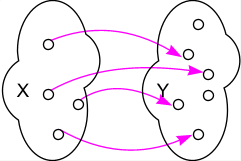
\includegraphics[scale=0.5]{injektiv.png}

\paragraph{Injektivität zeigen}
Injektiv wird meist direkt über die zweite Eigenschaft gemacht oder per Wiederspruchsbeweis (indirekter Beweis) mittels der ersten Eigenschaft bewiesen.
\todo{Beispiel?}

\paragraph{Eigenschaften}
\begin{itemize}
	\item Die Gleichung $f(x) = y$, $f$ ist injektiv und $y$ gegeben, verfügt über eine oder keine Lösung für $x$
	\item Eine \textit{stetige reelwertige} Funktion auf einem \textit{reelen Intervall} ist genau dann \underline{injektiv}, wenn sie in ihrem gesamten Definitionsbereich \textit{streng monoton} steigend oder fallend ist.
	\item Sind die beiden Funktionen $g, f$ injektiv, so ist die \underline{Komposition} $g \circ f$ ebenfalls injektiv
	\item Ist $g \circ f$ injektiv, so ist $f$ injektiv
	\item $f: M \rightarrow N$ ist injektiv, wenn es die \underline{links inverse} Funktion $g: N \rightarrow M$ gibt, so dass $g \circ f = \id_M$
\end{itemize}

\subsubsection{Surjektiv}
Sei $f: M \rightarrow N$, $f$ ist surjektiv, wenn folgendes gilt:
\begin{align*}
\forall y \in N: \exists x \in M: f(x) = y
\end{align*}
Wenn also für jedes Element aus $N$ mindestens ein (können auch mehr sein) Element in $M$ gibt, dass auf das Element aus $N$ zeigt.

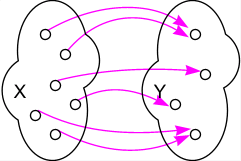
\includegraphics[scale=0.5]{surjektiv.png}

\paragraph{Eigenschaften}
\begin{itemize}
	\item Die Gleichung $f(x) = y$, $f$ ist surjektiv und $y$ gegeben, verfügt über eine oder mehrere Lösungen für $x$.
	\item Sind die Funktionen $f: A \rightarrow B$ und $g: B \rightarrow C$ surjektiv, so ist die \underline{Komposition} $g \circ f: A \rightarrow C$ auch surjektiv
	\item Ist $g \circ f$ surjektiv, so folgt, dass $g$ surjektiv ist
	\item $f: A \rightarrow B$ ist genau dann surjektiv, wenn $f$ ein \underline{rechtes Inverse} hat, also $g: B \rightarrow A$ mit $f \circ g = \id_B$
\end{itemize}

\subsubsection{Bijektiv}
Eine Funktion ist bijektiv, wenn sie injektiv und surjektiv ist.

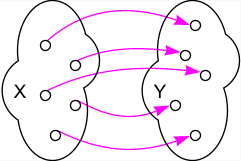
\includegraphics[scale=0.5]{bijektiv.png}

\paragraph{Eigenschaften}
\begin{itemize}
	\item Es gelten die Eigenschaften von Injektivität und Surjektivität
	\item Die Gleichung $f(x) = y$, $f$ ist bijektiv und $y$ gegeben, verfügt über genau eine Lösung für $x$
	\item Sind die Funktionen $f: A \rightarrow B$ und $g: B \rightarrow C$ bijektiv, dann ist auch die \underline{Komposition} $g \circ f: A \rightarrow C$ bijektiv.
	\item Ist $g \circ f$ bijektiv, dann ist $f$ injektiv und $g$ surjektiv
\end{itemize}

\section{Zwischenwertsatz}
Sei $f: [a,b] \to \R$ eine stetige reele Funktion, die auf einem Intervall
definiert ist. Dann existiert zu jedem $u \in [f(a), f(b)]$ (falls $f(a) \leq
f(b)$, sonst $u \in [f(b), f(a)]$) ein $c \in [a,b]$, sodass gilt: $f(c)= u$.

\subsection{Beispiel (Fixpunkt)}
Sei $f: [0,1] \to [0,1]$. Zeige: $f$ hat einen Fixpunkt, d.h. es gibt ein $x
\in [0,1]$ derart, dass $f(x) = x$.

Man erzeugt die Funktion $g: [0,1] \to \R, g(x) := f(x) - x$. Es gilt: $f(x) =
x \Leftrightarrow g(x) = 0$, d.h. ein Punkt x ist genau dann ein Fixpunkt von
$f$ wenn er eine Nullstelle von $g$ ist. Es ist zu zeigen, dass $g$ immer eine
Nullstelle auf $[0,1]$ hat. Als Differenz von zwei stetigen Funktionen ist $g$
stetig. Weil ausserdem $f(x) \in [0,1] \; \forall x \in [0,1]$ gilt, ist $g(0)
\geq 0 \geq g(1)$. Da $g$ stetig ist, gibt es daher nach dem Zwischenwertsatz
ein $x \in [0,1]$ mit $g(x) = 0$ und somit gibt es $f(x) = x$.

\section{Folgen in $\R$}

\subsection{Definitionen}
\begin{description}
  \item[konvergent] $\lim_{x \to \infty} a_n$ existiert \index{konvergent}
  \item[divergent] $\lim_{x \to \infty} a_n$ existiert nicht \index{divergent}
  \item[Nullfolge] $\lim_{x \to \infty} a_n = 0$ gilt \index{Nullfolge}
  \item[beschränkt] Es gibt $C_1, C_2$, so dass gilt $C_1 \leq a_n \leq C_2$
  bzw. $C$ gibt, so dass $|a_n| \leq C$
  \item[unbeschränkt] falls $(a_n)$ nicht beschränkt ist. Unbeschränkte folgen
  sind stets \underline{divergent}
  \item[monoton wachsend] $a_n \leq a_{n+1} \quad \forall n \in \N$ \index{monoton}
  \item[streng monoton wachsend] $a_n < a_{n+1} \quad \forall n \in \N$
  \item[monoton fallend] $a_n \geq a_{n+1} \quad \forall n \in \N$
  \item[streng monoton fallend] $a_n > a_{n+1} \quad \forall n \in \N$
  \item[alternierend] die Vorzeichen der Folgenglieder wechseln sich ab
  \item[bestimmt divergent / uneigentlich konvergent] es gilt $\lim_{n \to
  \infty} a_n = \pm \infty$
\end{description}

\begin{definition}[Grenzwert] \index{Grenzwert}
	\begin{align*}
		\lim_{n \to \infty} a_n = a & \Leftrightarrow a_n \to a \\
		& \Leftrightarrow \forall \epsilon > 0 \exists n_0 \in \N \forall n \geq n_0:
		|a_n - a| < \epsilon
	\end{align*}
\end{definition}

\begin{definition}[Teilfolge] \index{Teilfolge}
Werden von einer Folge beliebig viele Glieder weggelassen, aber nur so viele,
dass noch unendlich viele übrigbleiben, so erhält man eine Teilfolge.
\end{definition}

\begin{definition}[Häufungspunkt] \index{Häufungspunkt}
	$a$ ist Häufungspunkt der Folge $(a_n)$, wenn in jeder Umgebung von $a$
	unendlich viele Folgeglieder liegen. Das ist äquivalent damit, dass $a$ der
	Limes einer Teilfolge von $(a_n)$ ist.
\end{definition}

\begin{definition}[Limes superior / Limes inferior] \index{$\limsup$}\index{$\liminf$}
	Ist $(a_n)$ eine beschränkte Folge, so heisst der grösste Häufungspunkt Limes
	superior ($\limsup_{n \to \infty} a_n$ oder $\overline{\lim}_{n \to \infty}
	a_n$). Der kleinste Häufungspunkt ist der Limes inferior ($\liminf_{n \to
	\infty} a_n$ oder $\underline{\lim}_{n \to \infty} a_n$)
\end{definition}

\subsection{Rechnen mit Eigenschaften}
Addition:
\begin{itemize}
  \item $(a_n), (b_n)$ konvergiert $\Rightarrow (a_n + b_n)$ konvergiert
  \item $(a_n)$ konvergiert, $(b_n)$ divergent $\Rightarrow (a_n + b_n)$
  divergent
  \item $(a_n)$ beschränkt, $(b_n)$ beschränkt $\Rightarrow (a_n + b_n)$
  beschränkt
  \item $(a_n)$ beschränkt, $(b_n)$ unbeschränkt $\Rightarrow (a_n + b_n)$
  unbeschränkt
  \item $(a_n)$ beschränkt, $(b_n) \to \pm \infty \Rightarrow (a_n + b_n) \to
  \pm \infty$
  \item $(a_n) \to \infty$, $(b_n) \to \infty \Rightarrow (a_n + b_n) \to \infty$
  \item $(a_n) \to -\infty$, $(b_n) \to -\infty \Rightarrow (a_n + b_n) \to
  -\infty$
\end{itemize}

Produkt:
\begin{itemize}
  \item $(a_n)$ Nullfolge, $(b_n)$ beschränkt $\Rightarrow (a_n b_n)$ Nullfolge
  \item $(a_n)$ konvergent, $(b_n)$ beschränkt $\Rightarrow (a_n b_n)$
  beschränkt
  \item $(a_n)$ konvergent, $(b_n)$ konvergent $\Rightarrow (a_n b_n)$
  konvergent
  \item $(a_n)$ konvergent gegen $a \neq 0$, $(b_n)$ divergent $\Rightarrow
  (a_n b_n)$ divergent
\end{itemize}

\subsection{Rechnen mit Grenzwerten}
$\lim_{n \to \infty} a_n = a$, $\lim_{n \to \infty} b_n = b$\\
\emph{\underline{Achtung!} Untenstehendes gilt \underline{nur} wenn die Grenzwerte von $a_n$ und $b_n$ existieren. (Nicht $0$ oder $\inf$ sind.)}
\begin{itemize}
  \item $\lim_{n \to \infty} (a_n \pm b_n) = a \pm b$
  \item $\lim_{n \to \infty} (c \cdot a_n) = c \cdot a$
  \item $\lim_{n \to \infty} (a_n b_n) = ab$
  \item \underline{Achtung:} $\lim_{n \to \infty} (a_n)^c = (\lim_{n \to
  \infty} a_n)^c$, nur wenn $c \neq n$
  \item $\lim_{n \to \infty} \frac{a_n}{b_n} = \frac{a}{b}, \quad (b_n)$ keine
  Nullfolge
\end{itemize}

\subsection{Hilfsmittel}
\textbf{Bernoullische Ungleichung}: Für $x \geq -1$ und $n \in \N$
\[
	(1+x)^n \geq 1 + nx
\]


\textbf{Vergleich von Folgen}: weiter rechts stehende Werte gehen schneller nach
$\infty$
\[
	1, \quad \ln n, \quad n^\alpha \; (\alpha > 0), \quad q^n \; (q > 1), \quad n!,
	\quad n^n
\]

\textbf{Stirlingformel}:
\[
	n! \approx \sqrt{2 \pi n} \left (\frac{n}{e} \right )^n
	\Rightarrow \left ( \frac{n}{e} \right )^n \sqrt{2 \pi n} \leq n! \leq \left (
	\frac{n}{e} \right )^n \sqrt{2 \pi n} \cdot e^\frac{12}{n}
\]

\subsection{Konvergenzkriterien}\index{Konvergenzkriterien}
\begin{align*}
	a_n \to a \Leftrightarrow a_n - a \to 0 \Leftrightarrow |a_n - a| \to 0
\end{align*}
	
\begin{itemize}[leftmargin=*]	
	\item Ist $\lim_{n \to \infty} a_n = a$, so ist der Limes $a$ einziger
	Häufungspunkt der Folge $(a_n)$ und jede Teilfolge konvergiert auch gegen $a$.
	
	\textbf{Beispiel:} Wegen $\left( 1 + \frac{1}{n} \right)^n \to e$, so gilt auch
	$\left( 1 + \frac{1}{2n} \right)^{2n} \to e$
	
	\item Hat die Folge zwei verschiedene Häufungspunkte, so ist die Folge sicher
	divergent.
	
	\item Ist die Folge monoton steigend und nach oben beschränkt, dann existiert
	$\lim_{n \to \infty} a_n$. Ist die Folge monoton fallend und nach unten
	beschränkt, dann existiert $\lim_{n \to \infty} a_n$
	
	\item Konvergiert $\sum_{n=0}^\infty a_n$, so ist $\lim_{n \to \infty} a_n =
	0$\\
	Damit kann die Regeln für Reihen verwenden. Siehe Grenzwerte von Reihen.
	
	\item Gibt es eine Funktion $f$ mit $f(n) = a_n$ und $\lim_{x \to \infty} f(x)
	= a$, so gilt auch $\lim_{n \to \infty} a_n = a$.\\
	Damit kann man zum Beispiel die Regel von \underline{l'Hospital} und die
	restlichen Methoden anwenden. Siehe Grenzwerte von Funktionen.\\
	\underline{Achtung:} Es kann sein, dass $f$ keinen Grenzwert besitzt, aber
	$(a_n)$ schon.
	
	\item \textbf{Einschliessungskriterium}: Sind $(a_n), (b_n), (c_n)$ Folgen mit
	$a_n \leq b_n \leq c_n$ und haben $(a_n), (c_n)$ den gleichen Grenzwert $a$, so
	konvergiert auch $(b_n)$ nach $a$.
\end{itemize}

\subsection{Tipps \& Beispiele}
\subsubsection{Brüche}
$\lim_{n \to \infty} \frac{n^2 + \ln n}{\sqrt{n^4 - n^3}}$

Bei Brüchen empfiehlt es sich den am stärksten wachsenden Teil (das am
schnellsten wachsende $n$) zu kürzen. In diesem Fall ist es das $n^4$ in der
Wurzel, also $n^2$.

\begin{align*}
\ldots &= \lim_{n \to \infty} \frac{n^2 + \ln n}{\sqrt{n^4 - n^3}}
\cdot \frac{\frac{1}{n^2}}{\frac{1}{n^2}} = \lim_{n \to \infty} \frac{n^2 + \ln
n}{n^2 \sqrt{1 - \frac{1}{n}}} \cdot \frac{\frac{1}{n^2}}{\frac{1}{n^2}} \\
&= \lim_{n \to \infty} \frac{1 + \frac{\ln n}{n^2}}{\sqrt{1 - \frac{1}{n}}}
= \frac{1 + 0}{\sqrt{1 - 0}} = 0
\end{align*}

\subsubsection{l'Hospital für Folgen (Folge als Funktion)}
$\lim_{n \to \infty} \frac{\ln n}{n^2}$

Die Funktion $f(x) = \frac{\ln x}{x^2}$ entspricht unseren Folgegliedern ($f(n)
= a_n = \frac{\ln n}{n^2}$). Für $n \to \infty$ hat der Nenner und der Zähler
den Grenzwert $\infty$, also wenden wir die Regel von l'Hospital an.

\begin{align*}
\ldots &= \lim_{x \to \infty} \frac{(\ln x)'}{(x^2)'} = \lim_{x \to \infty}
\frac{\frac{1}{x}}{2x} = \lim_{x \to \infty} \frac{1}{x^2} = 0
\end{align*}

Somit geht auch die Folge gegen 0.

\subsubsection{Wurzeln}
$\lim_{n \to \infty} (\sqrt{n^2 + an + 1} - \sqrt{n^2 + 1})$

Hier wendet man die dritte binomische Formel an, um den grenzwert zu berechnen.
Die einzelnen Terme streben jeweils gegen $\infty$ und $\infty - \infty$ kann
nicht berechnet werden.

\underline{Achtung} auf die Vorzeichen beim Anwenden der Regel!

\begin{align*}
&= \lim_{n \to \infty} (\sqrt{n^2 + an + 1} - \sqrt{n^2 + 1}) \cdot
\left(\frac{\sqrt{n^2 + an + 1} + \sqrt{n^2 + 1}}{\sqrt{n^2 + an + 1} +
\sqrt{n^2 + 1}} \right) \\
&= \lim_{n \to \infty} \frac{(n^2 + an + 1) - (n^2 + 1)}{\sqrt{n^2 + an + 1} +
\sqrt{n^2 + 1}} \\
&= \lim_{n \to \infty} \frac{an}{\sqrt{n^2 + an + 1} + \sqrt{n^2 + 1}} 
\end{align*}

nun verwenden wir den Tipp für Brüche und kürzen das $n$ heraus

\begin{align*}
\ldots &= \lim_{n \to \infty} \frac{a}{\sqrt{1 + \frac{a}{n} + \frac{1}{n^2}} +
\sqrt{1 + \frac{1}{n^2}}} = \frac{a}{1 + 1} = \frac{a}{2}
\end{align*}

\subsubsection{Laufvariable im Exponent}
$\lim_{x \to 0} (3 - |x|)^{\frac{\sin(x)}{x}}$\newline
$\Rightarrow (3 - |x|)^{\frac{\sin(x)}{x}} = e^{\frac{\sin(x)}{x} \cdot \ln(3 -
|x|)}$\newline
$\Rightarrow 
\lim_{x \to 0} (3 - |x|)^{\frac{\sin(x)}{x}} = \lim_{x \to 0}e^{\frac{\sin(x)}{x} \cdot \ln(3 -
|x|)}$\newline
$\Rightarrow \lim_{x \to 0}\frac{\sin(x)}{x}\cdot \ln(3-|x|) = \ln(3)$\newline
$\Rightarrow \lim_{x \to 0}(3 - |x|)^{\frac{\sin(x)}{x}} = e^{\ln(3)} = 3$


\subsubsection{Gruppieren}
%Aus Analysis II (2012) Serie 1 Aufgabe 2b
Hat man zum Beispiel die Folge $s_n = 1 + \frac{1}{3} + \frac{1}{5} + ... + \frac{1}{2n-1}$ so kann man die 
einzelnen Therme gruppieren und abschätzen in diesem Fall z.B. mit $\frac{1}{4}$ (zweiter Therm, dritter und vierter Therm,
fünfter bis achter Therm, nächste 8 Therme, etc.). Wir erhalten dann $s_{2^k} \geq 1 + \frac{k}{4}$ und sehen somit das die 
Reihe nicht beschränkt ist und somit auch nicht konvergiert.

\subsection{Cauchy-Folgen}\index{Cauchy-Folge}
\begin{definition}[Cauchy-Folge]
Sei $(a_n)_{n \in \N}$ eine Folge in $\R$. $(a_n)_{n \in \N}$ heisst \textbf{Cauchy-Folge}, falls gilt
\begin{align*}
\forall \epsilon > 0 \; \exists n_n = n_0(\epsilon) \in \N \; \forall n, l \geq n_0: |a_n - a_l| < \epsilon
\end{align*}
\end{definition}

Die Definition sagt grundsätzlich aus, dass ab einem $n_0(\epsilon)$ (also einem Anfang $n_0$, der abhängig von $\epsilon$ ist)
die Folgeglieder nur noch $\epsilon$ Abstand zu einander haben. Also der Abstand beliebig klein wird zwischen Folgegliedern.

\begin{satz}[Cauchy-Kriterium]
Für $(a_n)_{n \in \N} \subset \R$ sind äquivalent:
\begin{itemize}
	\item $(a_n)_{n \in \N}$ ist konvergent
	\item $(a_n)_{n \in \N}$ ist Cauchy-Folge
\end{itemize}
\end{satz}

\section{Reihen}

\subsection{Definitionen}
Eine Reihe $\sum_{n = 1}^\infty a_n$ ist \underline{konvergent} mit Grenzwert
$s$, wenn die Folge der \underline{Partialsummen} $(S_m)$, $S_m :=
\sum_{n=1}^m a_n$ gegen $s$ konvergiert. Also wenn gilt: $S_m \to s$.

\begin{definition}[$\epsilon$-Kriterium]
	$\forall \epsilon > 0 \; \exists n_0 \in \N \; \forall m \geq n_0: \left|
	\sum_{n=1}^m a_n - s \right| < \epsilon$
\end{definition}

\begin{definition}[Absolute Konvergenz]\index{Konvergenz}
Wenn auch die Reihe der Absolutbeträge $\sum_{n=1}^\infty |a_n|$ konvergiert, so
heisst die Reihe absolut konvergent. Aus der absoluten Konvergenz folgt
Konvergenz. Der Umkehrschluss ist nicht möglich.
\end{definition}

\subsection{Rechenregeln Reihen}
Für \underline{konvergente} Reihen gilt:
\[
	\sum_{n=1}^\infty a_n = A, \sum_{n=1}^\infty b_n = B \Rightarrow
	\sum_{n=1}^\infty (\alpha a_n + \beta b_n) = \alpha A + \beta B
\]

\subsection{Konvergenzkriterien}
\begin{tabular}{|l|}
\hline
	Konvergiert $\sum_{n=1}^\infty a_n$, so ist $\lim_{n \to \infty} a_n = 0$.\\
	Wenn also $\lim_{n \to \infty} a_n \neq 0$, so konvergiert die Reihe
	\underline{nicht}\\
\hline
\end{tabular}

\onecolumn

{\footnotesize
\begin{tabular}{|p{2cm}||p{3cm}|p{3cm}|p{3cm}|p{3cm}|p{3cm}|}
\hline & \multicolumn{4}{l}{schnelles Fallen} & langsames Fallen \\
\hline
 
wie schnell gehen die $a_n$ gegen 0 & exponentiell wie $q^n, |q| < 1$ &
polynominal wie $n^{-\alpha}, \alpha > 1$ & \multicolumn{2}{|c|}{höchstens wie
$1/n$} & gar nicht \\ \hline

Beispiele & \begin{align*} a_n = \frac{n^8}{2^n},\\ a_n =
(\sqrt[n]{n} - 1)^n,\\
a_n = \frac{1}{n!},\\ a_n = \left( \frac{-1}{4}\right)^n \end{align*} &
\begin{align*} a_n = \frac{1}{n^2}, \\ a_n = \frac{1}{n^{100}}, \\ a_n =
\frac{1}{(n + \ln n)^2}, \\ a_n = \frac{20}{n^2 - 33} \end{align*} &
\begin{align*} a_n = \frac{(-1)^n}{\ln n}, \\ a_n = \frac{(-1)^n}{n}
\end{align*} & \begin{align*} a_n = \frac{1}{\ln n}, \\ a_n = \frac{1}{n + \ln
n}, \\ a_n = \frac{1}{n} \end{align*} & \begin{align*} a_n = (-1)^n, \\ a_n =
\sin n, \\ a_n = n^2 \end{align*}\\ \hline

passende Konvergenzkriterien & Wurzel- und Quotientenkriterium & Integral- und
Verdichtungskriterium & Leibniz-Kriterium & & $a_n \not\to 0$ \\ \hline

Vergleichs-, Majoranten-, Minorantenkriterium & Vergleichen mit $q^n$ &
Vergleichen mit $n^{-\alpha}$ & kein Vergleich möglich & Vergleichen mit
$\frac{1}{n}$ & \\ \hline

Konvergenz-verhalten & \multicolumn{2}{c|}{absolute Konvergenz} & keine
absolute Konvergenz (einfach Konvergenz) & \multicolumn{2}{|c|}{Divergenz} \\
\hline

\end{tabular}
}

\begin{tabular}{|p{4cm}|p{15cm}|}\hline
\multicolumn{2}{|c|}{direkte Kriterien}\\ \hline

\textbf{Quotientenkriterium} & Gut für Reihen, die Fakultäten oder Glieder der
Form $a^n$ enthalten. Nicht auf Reihen anwendbar, in denen die Glieder nur wie
eine Potenz von $n$ fallen. \\ \hline

\textbf{Wurzelkriterium} & Gut in Reihen, deren Glieder $n$-te Potenzen sind,
zusammen mit der Stirlingformel oft auch bei Fakultäten anwendbar. \\ \hline

\textbf{Leibnizkriterium} & Nur für alternierende Reihen.\\ \hline

\textbf{Integralkriterium} & Anwendbar auf monotone Reihen.\\ \hline

\multicolumn{2}{|c|}{direkte Kriterien}\\ \hline

\textbf{Vergleichskriterium} & Ermöglicht es "`Störterme"' wegzulassen und so
einfachere Reihen zu untersuchen \\ \hline

\textbf{Verdichtungskriterium} & Bei monotonen Reihen anwendbar. Für Reihen mit
langsam fallenden Gliedern \\ \hline

\textbf{Majoranten- und Minorantenkriterium} & Ähnlich wie Vergleichskriterium.
Wird mit einer Reihe verglichen, deren Glieder stets kleiner oder grösser sind.
\\ \hline
\end{tabular}

\twocolumn

\subsubsection{Reihen Kriterien}
Achtung. Die nachfolgenden Kriterien sagen nur aus, ob die Reihen konvergiert
oder nicht. Sie sagen \underline{nicht} aus, gegen was sie konvergieren!

\paragraph{Quotientenkriterium}
\[
\left| \frac{a_{n+1}}{a_n} \right| \to q. \quad \text{Dann gilt} \begin{cases}
q < 1 & \Rightarrow \sum_{n=1}^\infty a_n \text{ konvergiert absolut} \\
q = 1 & \Rightarrow \text{keine Aussage}\\
q > 1 & \Rightarrow \sum_{n=1}^\infty a_n \text{ divergiert}
\end{cases}
\]

\paragraph{Wurzelkriterium}
\[
\sqrt[n]{\left | a_n \right |} \to q. \quad \text{Dann gilt} \begin{cases}
q < 1 & \Rightarrow \sum_{n=1}^\infty a_n \text{ konvergiert absolut}\\
q = 1 & \Rightarrow \text{keine Aussage}\\
q > 1 & \Rightarrow \sum_{n=1}^\infty a_n \text{ divergiert}
\end{cases}
\]

\paragraph{Leibnizkriterium}
Wenn gilt:
\begin{itemize}
  \item $(a_n)$ ist alternierende Folge, d.h die Vorzeichen wechseln jedes Mal
  \item $a_n \to 0$ oder $|a_n| \to 0$
  \item $(|a_n|)$ ist monoton fallend
\end{itemize}
\ldots dann konvergiert $\sum_{n=1}^\infty a_n$

\paragraph{Majorantenkriterium}
Ist $|a_n| \leq b_n$ und $\sum_{n=1}^\infty b_n$ konvergent, so konvergiert
$\sum_{n=1}^\infty a_n$ absolut.

\paragraph{Minorantenkriterium}
Ist $a_n \geq b_n \geq 0$ und $\sum_{n=1}^\infty b_n$ divergent, so divergiert
$\sum_{n=1}^\infty a_n$

\subsection{Potenzreihe}
Die Potenzreihe hat die allgemeine Form
\[
\sum_{n=0}^\infty a_n (x - x_0)^n
\]

$x_0$ ist der Entwicklungspunkt der Potenzreihe und $(a_n)_{n \in \N}$ eine
beliebige Folge.

\subsubsection{Konvergenzradius}
Die Berechnung des Konvergenzradius ist für solche Reihen einfacher, da der
Faktor $(x - x_0)$ nicht analysiert werden muss. Entsprechend gilt für den
Konvergenzradius $r$:
$r = \frac{1}{\limsup_{n\to\infty} \sqrt[n]{\|a_n\|}}$ (Wurzelkriterium) bzw.
$r = \lim_{n\to\infty} \left | \frac{a_n}{a_{n+1}} \right |$
(Quotientenkriterium).

\section{Taylorreihe / -entwicklung}
Funktionen werden in der Umgebung eines bestimmten Punktes durch eine
Potenzreihe dargestellt. Damit wird die ursprüngliche Funktion angenähert.

Die Taylorreihe der Funktion $f$ mit Grad $m$ um den Punkt $a$ ist:
$T_m f(x;a) = \sum_{n = 0}^m \frac{f^{(n)}(a)}{n!}(x - a)^n$\newline
{\small
$= f(a) + \frac{f'(a)}{1!}(x-a) + \frac{f''(a)}{2!}(x-a)^2 +
\frac{f^{(3)}(a)}{3!}(x-a)^3 + \frac{f^{(4)}(a)}{4!}(x-a)^4\ldots$
}

Dabei ist $n! = 1 \cdot 2 \cdot 3 \cdot \ldots \cdot n$

\subsection{Rechenregeln}
\subsubsection{Addition}
$f, g$ sind $m$-mal differenzierbar:

$T_m (f + g)(x;a) = T_m f(x;a) + T_m g(x;a)$

\subsubsection{Multiplikation}
$f, g$ sind $m$-mal differenzierbar:

$T_m (f \cdot g)(x;a) = T_m(T_m f(x;a) \cdot T_m g(x;a))$

\underline{Achtung}: Anschaulich bedeutet es folgendes: Man
multipliziert die beiden Taylorreihen von $f$ und $g$ miteinander ($T_m f(x;a) \cdot T_m g(x;a)$).
Danach entfernt man alle Terme der Ordnung $> m$.

\subsubsection{Kettenregel}
$f: A \to B, g: B \to \R$ zwei $m$-mal differenzierbare Funktionen.
Entwickelt wird um den Punkt $a \in A$ mit $f(a) = q$ ($q$ muss man berechnen).
Dann gilt:
\begin{align*}
T_m (g \circ f)(x;a) &= T_m (f(g))(x;a)\\
&= T_m(T_m(g)(x;q) \circ (T_m(f)(x;a) - q))
\end{align*}

\subsubsection{Bemerkungen / Eigenschaften / Konvergenz}
\begin{itemize}
	\item Der Konvergenzradius kann 0 sein
	\item Falls Taylor-Reihe konvergiert, dann ist sie nicht notwendig gleich
	der Funktion, die sie beschreibt. Gegenbeispiel:
	$f(x) = \begin{cases}
	e^{-\frac{1}{x}} & x > 0\\
	0 & x \leq 0\end{cases}$
	\item Ist $f$ eine Potenzreihe, dann ist diese Potenzreihe auch die Taylor-Reihe
\end{itemize}
\section{Stetigkeit und Limes einer Funktion}
$\lim_{x \to a} f(x) = b$ bedeutet, dass die Funktion $f$ für $x \to a$ den
Grenzwert $b$ hat. Der Funktionswert nähert sich also immer näher an $b$ heran,
wenn $x$ sich $a$ annähert (Epsilon-Delta-Kriterium).
\[
\forall \epsilon > 0 \; \exists \delta > 0: \|x -a\| < \delta \Rightarrow
\|f(x) - f(a)\| < \epsilon
\]

Funktionsfolgen verhalten sich desweiteren wie Folgen. Es gelten also die
gleichen Eigenschaften.

\subsection{(Punktweise) Stetigkeit}
Die Definition für punktweise Stetigkeit ist die gleiche, wie die für
$\lim_{x \to a} f(x) = b$ (siehe die Definition gerade über diesem Kapitel).

Charakterisierungen der Stetigkeit von $f$ im Punkt $a$:
\begin{itemize}
	\item $\lim_{x \to a} f(x) = f(a)$ ist die Definition
	\item Man kann $\lim_{x \to a} f(x)$ auch als $f(\lim_{x \to a} x)$ schreiben.
	Also die Reihenfolge zwischen Bildung des Grenzwertes und der Anwendung der
	Funktion vertauschen. Beispiel: $\lim_{x \to \infty} \sin\frac{1}{x} =
	\sin(\lim_{x \to \infty} \frac{1}{x}) = \sin(0) = 0$
	\item Es gilt linker Grenzwert = Funktionswert = rechter Grenzwert: $\lim_{x
	\nearrow a} f(x) = f(a) = \lim_{x \searrow a} f(x)$
	\item Für eine beliebige (jede) Folge $(x_n)$ mit $x_n \to a$ hat $f(x_n) \to
	f(a)$ zu gelten. Dies ist praktisch um zu zeigen, dass eine Funktion an einer
	Stelle nicht stetig ist.
\end{itemize}

Eine Funktion $f$ ist stetig, wenn sie in allen Punkten stetig ist
(``punktweise Stetigkeit'').

Es gelten folgenden Eigenschaften:
\begin{itemize}
	\item Ist $f$ und $g$ stetig in einem gemeinsamen Definitionsbereich, so sind
	$f + g, f- g, f \cdot g, \frac{f}{g}, f \circ g$ ebenfalls stetig.
\end{itemize}

\subsection{Gleichmässige Stetigkeit}
Sei $f: D \to \R$, $D \subseteq \R$, dann ist $f$ genau dann stetig wenn gilt:
\[
\forall \epsilon > 0 \exists \delta > 0 \forall x,x_0 \in D: |x - x_0| < \delta
\Rightarrow |f(x) - f(x_0)| < \epsilon
\]

Der Unterschied zur punktweisen Stetigkeit liegt darin, dass $\delta$ und
$\epsilon$ nicht auch noch von $x_0$ abhängig sind. So ist $f(x) = x^2$ zwar
(punktweise) stetig, aber nicht gleichmässig stetig. Begründung: Je weiter
rechts man zwei Punkte mit einem Abstand kleiner als $\delta$ wählt, desto
grösser wird der Abstand der beiden Funktionswerte. Dieser Abstand der
Funktionswerte müsste aber kleiner als das vorgegebene $\epsilon$ bleiben.

\subsection{Lipschitz-Stetigkeit}
Eine Funktion $f: \R \to \R$ ist Lipschitz-stetig, wenn eine Konstante $L$
existiert, so dass gilt:
\[
\forall x_1,x_2 \in \R: \|f(x_1) - f(x_2)\| \leq L \cdot \|x_1 - x_2\|
\]

\subsection{Stetigkeit, Differenzierbarkeit, Integrierbarkeit}
Sei $f$ eine Funktion, so gilt:

$f$ differenzierbar $\Rightarrow$ $f$ stetig $\Rightarrow$ $f$ integrierbar\\
\\
$f$ \emph{nicht} integrierbar $\Rightarrow$ $f$ \emph{nicht} stetig $\Rightarrow$ $f$\emph{nicht} differenzierbar  

\subsection{Abhängigkeit der Stetigkeitsbegriffe}
Sei $f$ eine reelle Funktion, so gilt:

$f$ Lipschitz-stetig $\Rightarrow$ $f$ absolut stetig $\Rightarrow$ $f$
gleichmässig stetig $\Rightarrow$ $f$ (punktweise) stetig.

\subsection{Regel von de l'Hospital}
Sei $a \in \R \cup \{\infty, -\infty\}$. Es hat zu gelten:
\begin{itemize}
  \item $\lim_{x \to a} f(x) = \lim_{x \to a} g(x) = 0 \text{ oder } \pm\infty$
  \item In der Nähe von $a$ ist $g'(x) \neq 0$
\end{itemize}

Dann ist
\[
\lim_{x \to a} \frac{f(x)}{g(x)} = \lim_{x \to a}
\frac{f'(x)}{g'(x)}
\]

Diese Regel kann man mehrfach anwenden hintereinander. \underline{Achtung:} Es
kann sein, dass der Limes $\lim_{x \to a} \frac{f'(x)}{g'(x)}$ nicht existiert,
aber von $\lim_{x \to a} \frac{f(x)}{g(x)}$ trotzdem.


\subsection{Tips zur Stetigkeit}
\begin{itemize}
  \item Um zu zeigen das eine Funktion mit mehreren Parameter in einem Punkt \emph{nicht} stetig ergänzbar ist
	hilft es häufig die Parameter gleich zu setzen. (Häufig geht dann der Limes nicht gegen den gesuchten Punkt
	 $\Rightarrow$ die Funktion ist \emph{nicht} stetig ergänzbar.)
\end{itemize}

\section{Funktionsfolgen}
\subsection{Definition}
Eine Funktionsfolge $(f_n)$ \underline{konvergiert punktweise} auf dem
Definitionsbereich $I$ gegen $f$, wenn für jedes $x \in I$ gilt $f_n(x) \to f(x)$.
\[
\forall \epsilon > 0 \; \forall x \in I \; \exists n_0 \in \N: n \geq n_0
\Rightarrow |f(x) - f_n(x)| < \epsilon
\]

Die Folge \underline{konvergiert gleichmässig} auf $I$ gegen $f$, wenn
$\sup_{x\in I} |f_n(x) - f(x)| \to 0$ gilt. Das bedeutet, dass die obere
Definition für alle $x$ \underline{dasselbe} $n_0$ verwendet und nicht jeweils
verschiedene:
\[
\forall \epsilon > 0 \; \exists n_0 \in \N \; \forall x \in I: n \geq n_0
\Rightarrow |f(x) - f_n(x)| < \epsilon
\]

\underline{Wichtig}: gleichmässige Konvergenz $\Rightarrow$ punktweise
Konvergenz. Nicht aber andersrum!

\section{Differenzierbarkeit}
\subsection{Definition}
$f$ ist in $a \in I$ differenzierbar mit der Ableitung $f'(a)$, wenn
\[
\lim_{x \to a} \frac{f(x) - f(a)}{x - a} =: f'(a) = \frac{d}{dx}f(a)
\]
existiert.

Ist $f'$ stetig im Definitionsbereich, so heisst $f$ stetig differenzierbar. Man
kann also $f$ differenzieren und bekommt mit $f'$ eine stetige Funktion. Es gilt
auch $f \in C^1(I)$. $C^n(I)$ ist die Menge der $n$-mal stetig differenzierbaren
Funktionen über dem Intervall $I$.

\subsection{Mittelwertsatz (Satz von Lagrange)}
Ist $f$ au $[a,b]$ stetig und in $]a, b[$ differenzierbar, so gibt es ein $c
\in ]a,b[$ mit
\[
\frac{f(b) - f(a)}{b-a} = f'(c)
\]

\subsubsection{Beispiel: Ungleichungen}
Zu zeigen: $e^x(y-x) < e^y - e^x < e^y(y-x), \; \forall x < y$:


Der Mittelwertsatz wird auf die Exponentialfunktion angewendet. Damit gilt für
ein Paar von Zahlen $x < y$ ein $u \in ]x,y[$, für welches gilt: $\frac{e^y
- e^x}{y-x} = e^u$. Weil die Exponentialfunktion in $\R$ streng monoton wachsend
ist, gilt $e^x < e^u < e^y$ und somit gilt: $e^x < \frac{e^y-e^x}{y-x} < e^y$.
Multipliziert man nun mit dem Nenner des Bruchs bekommt man: $e^x (y-x) < e^y -
e^x < e^y(y-x)$.

\subsection{Monotonie}
\begin{itemize}
	\item $f' > 0 \Rightarrow f$ streng monoton steigend
	\item $f' \geq 0 \Leftrightarrow f$ monoton steigend
	\item $f' < 0 \Rightarrow f$ streng monoton fallend
	\item $f' \leq 0 \Leftrightarrow f$ monoton fallend
\end{itemize}

\subsubsection{Extremstellen}
\begin{itemize}
	\item $f'(x_0) = 0, f''(x_0) > 0 \Rightarrow$ Minimum bei $x_0$
	\item $f'(x_0) = 0, f''(x_0) < 0 \Rightarrow$ Maximum bei $x_0$
	\item $f''(x_0) = 0, f'''(x_0) \neq 0 \Rightarrow$ Wendepunkt in $x_0$
	\item $f'(x_0) = 0, f''(x_0) = 0, f'''(x_0) \neq 0 \Rightarrow$ Sattelpunkt in
  	$x_0$
	\item Extrema bei $x_0 \Rightarrow f'(x_0) = 0$
\end{itemize}

\subsection{Zusammenhang zwischen Stetigkeit und Differenzierbarkeit}
\begin{itemize}
	\item differenzierbar $\Rightarrow$ stetig
	\item differenzierbar $\not\Leftarrow$ stetig
\end{itemize}

\subsection{Umkehrsatz}
% aus http://mathematik-netz.de/pdf/Umkehrsatz.pdf
Ist $f:I \to \R$ auf I differenzierbar mit $f'(x)>0$ für jedes $x \in I$, 
so ist $f$ streng monoton wachsend und damit injektiv, die Umkehrfunktion $f^{-1}:f(I) \to I$ existiert und ist ebenfalls streng monoton wachsend,
die Ableitung $(f^{-1})'(y)$ existiert für alle $y \in f(I)$ mit $f'(f^{-1}(y)) \neq 0)$, und zwar gilt dann \[
(f^{-1})'(y) = \frac{1}{f'(f^{-1}(y))}
\]

\section{Partialbruchzerlegung}
Mit dieser Methode wird ein schwieriger Bruch in eine Summe von einfacheren
Brüchen zerlegt. Damit lässt sich der ursprüngliche Bruch einfacher integrieren.

\begin{enumerate}
	\item Den Grad des Zählers und des Nenners vergleichen von $R$
	\begin{enumerate}
		\item Ist der Zählergrad (über Bruchstrich) grösser oder gleich dem Nennergrad
		(unter Bruchstrich), so dividiert man den Zähler durch den Nenner. Man erhält
		daraus das Polynom $P^*$ und möglicherweise einen Rest $R$, sodass gilt: $R =
		P + R^*$.
		\item Ist $R^* \equiv 0$, so ist das Verfahren abgeschlossen. Sonst arbeitet
		man nun mit dem Rest $R^*$ weiter als Bruch, den man ansieht.
	\end{enumerate}
	\item Man berechnet die Nullstellen vom Nenner des Bruches.
	\item Nun setzt man den ursprünglichen Bruch gleich der Summe der
	Partialbrüche. Die Partialbrüche sind jeweils abhängig von den Nullstellen:
	\begin{enumerate}
		\item Für jede einfache reelle Nullstelle $x_i$ ist der Summand
		$\frac{a_{i1}}{x-x_i}$ zu nehmen
		\item Für jede $r_i$-fache Nullstelle $x_i$ erhält man $r_i$ Summanden:
		$\frac{a_{i1}}{x-x_i} + \frac{a_{i2}}{(x-x_i)^2} + \ldots +
		\frac{a_{ir_i}}{(x-x_i)^{r_i}}$
	\end{enumerate}
	\item Nun berechnet man die unbekannten $a_{ij}$ indem man die Partialbrüche
	gleichnamig macht und dann die Koeffizienten des ursprünglichen Zählers mit
	denen des gleichnamigen Bruchs vergleicht.
\end{enumerate}

\subsection{Beispiel}
$R(x) = \frac{x^2}{x^2-2x+1}$.

Der Zählergrad ist gleich dem Nennergrad,
weswegen wir eine Polynomdivision durchführen: $\Rightarrow R(x) = 1 +
\frac{2x-1}{(x-1)^2}$.

Aus $(x-1)^2$ folgt, das wir nur eine Nullstelle haben $x_0 = 1$. Es handelt
sich dabei um eine doppelte Nullstelle.

Somit gilt:
\begin{align*}
\frac{2x-1}{(x-1)^2} &= \frac{a_1}{x-1} + \frac{a_2}{(x-1)^2}\\
2x-1 &= a_1(x-1) + a_2\\
2x-1 &= a_1 x - a_1 + a_2
\end{align*}
Daraus folgt, dass $a_1 = 2$ und $a_2 = 1$ (lineares Gleichungssystem).

Somit gilt: $R(x) = \frac{x^2}{x^2-2x+1} = 1 + \frac{2}{x-1} +
\frac{1}{(x-1)^2}$

\section{Integralrechnung}
\subsection{Berechnung}
$\int \alpha f(x) + \beta g(x)\,dx = \alpha \int f(x)\,dx + \beta \int g(x)\,dx$

\subsubsection{Substitutionsregel}
$\int F'(g(x)) g'(x)dx = F(g(x))$


\begin{enumerate}
	\item Für die neue Variable $u = g(x)$ bildet man: $\frac{du}{dx} = g'(x)
	\Leftrightarrow du = g'(x)dx$. Ersetzt also $g(x) = u$ und $dx =
	\frac{du}{g'(x)}$. Wenn noch $x$ übrig sind, ist ein Zwischenschritt nötig:
	Löse $u = g(x)$ durch $x = h(x)$ nach $x$ auf und ersetze die restlichen $x$
	durch $h(x)$.
	\item Bei bestimmten Integralen: Sei $int_a^b \ldots \,dx$. Dann sind die neuen
	Grenzen für das neue Integral $g(a)$ und $g(b)$
	\item Berechne das Integral in $u$
	\item Ersetze im Ergebnis $u$ durch $g(x)$
\end{enumerate}

\paragraph{Beispiel 1}
Das Integral $\int_{-2}^1 x^2 \,dx$ berechnet die blaue Fläche die durch die Funktion $f(x) = x^2$ beschränkt wird.
$F(x)$ sei die Stammfunktion von $f(x)$,  generell berechnen wir $\int x^y \,dx = \frac{x^{(y+1)}}{y+1}$, somit $F(x) = \frac{x^3}{3}$.
Somit $\int_{-2}^1 x^2 \,dx = F(x) \left |_{-2}^1 \right. = F(1) - F(-2) =  \frac{1^3}{3} -  \frac{-2^3}{3} = \frac{1}{3} +  \frac{8}{3} = 3.$

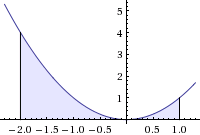
\includegraphics[scale=1]{integral_x2.png}

\paragraph{Beispiel 2}
$\int_0^2 x \sqrt{x+1}^3 \,dx$

Die Wurzel wird substituiert: $u = g(x) = \sqrt{x+1}$.

\begin{enumerate}
	\item $\frac{du}{dx} = g'(x) = \frac{1}{2\sqrt{x+1}} = \frac{1}{2u}$. Somit
	wird $\sqrt{x+1}^3$ durch $u^3$ ersetzt und $dx$ durch
	$\frac{du}{\frac{1}{2}u} = 2u\,du$. Im Integral wären somit die Wurzel und das
	$dx$ ersetzt. Es bleibt noch das $x$ übrig vor der Wurzel. Lösen wird
	$\sqrt{x+1} = u$ nach $x$ auf, so erhalten wir $x = u^2 - 1$.
	\item Neue Grenzen: $g(0) = 1$ und $g(2) = \sqrt{3}$
	\item $\int_0^2 x \sqrt{x+1}^3 \,dx = \int_1^{\sqrt{3}} (u^2 - 1)u^3 2u \,du =
	2\int(u^6 -u^4) \,du = [\frac{2}{7}u^7 - \frac{2}{5}u^5]_{1}^{\sqrt{3}}$
	\item Rücksubstitution: $\int_0^2 x \sqrt{x+1}^3 \,dx =
	[\frac{2}{7}\sqrt{x+1}^7 - \frac{2}{5}\sqrt{x+1}^5]_{1}^{\sqrt{3}} = \ldots = \frac{144}{35}\sqrt{3} +
	\frac{4}{35}$
\end{enumerate}
\section{Riemannsummen (Riemannintegral)}
\subsection{Riemansumme}
Wir betrachten die folgende Einteilung des Intervals $[a,b]$:\[
E: [a,b] = \bigcup_{k=1}^{N}[x_{k-1}, x_k] \text{ mit } x_k = a + k \cdot \frac{b-a}{N}.
\]
Die Feinheit dieser Zerlegung ist:\[
\delta(E) \equiv max\{x_k - x_{k-1}|k = 1...N\} = \frac{b-a}{N} \xrightarrow{N \to \infty} = 0
\]
$\xi_i$ sein ein Punkt auf dem Interval $[x_{i-1}, x_i]$, somit $\xi_i \in[x_{i-1}, x_i]$.\\

\begin{figure}
	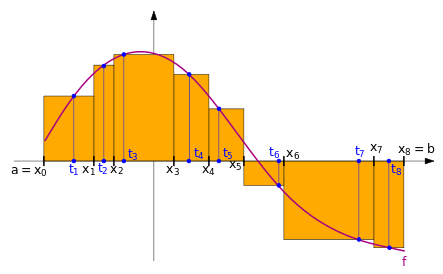
\includegraphics[width=\columnwidth]{riemann.png}
	\caption[Bildunterschrift]{Darstellung Riemannintegral mit $\xi_i = t_i$ und unsymetrischer Intervaleinteilung $E$.}
\end{figure}

Somit können wir die Riehmannsumme bilden:
\begin{align*}
\int_a^b f(x)\;dx &=\sum (f,E,\xi)\\
&= \lim_{N \to \infty} \underbrace{\sum_{k=0}^{N-1}
\underbrace{f(\xi_i)}_{\text{``Höhe''}} \cdot
\underbrace{\delta(E)}_{\text{``Länge''}}}_{\text{Riemann-Summe}}\\
&= \lim_{N \to \infty} \sum_{k=0}^{N-1} {f(a +
k\frac{b-a}{N})} \cdot \frac{b-a}{N}
\end{align*}


\subsection{Riemann Integrabel}
Die Funktion $f$ sei Riemann Integrabel wenn es ein $I \in \R$ gibt so dass: $\forall \epsilon > 0, \exists \nu > 0$ so dass \[
|I| - \epsilon < \sum (f,E,\xi) < |I| + \epsilon
\]
für jede Einteilung $E$ von $[a,b]$ mit $\delta(E) < \nu$, und für jede Wahl von Zwischenpunkten $\xi$.

\subsection{Beispiel}
Es soll das Intergral mittels Riemannschen Summe berechnet werden: $\int_a^b
e^{\lambda x}\,dx, \; \lambda \in \R$. $f(x) = e^{\lambda x}$

Zuerst unterteilt man das Intervall $[a,b]$: $E: [a,b] =
\bigcup_{k=1}^N[c_{k-1}, c_k]$ mit $c_k = a + k\cdot \frac{b-a}{N}$.

Die Feinheit dieser Zerlegung ist somit $\delta(E) = \max\{c_k - c_{k-1} | k =
1 \ldots N\} = \frac{b-a}{N}$. Dabei gilt $\delta(E) = \frac{b-a}{N} \to 0$ ($N
\to \infty$). Dies ist wichtig. Wir müssen die Feinheit unglaublich klein
bekommen können, also nahezu $0$. Je feiner die Feinheit desto genauer wird
unsere Riemann'sche Summe. Der Grenzwert dieser Summe für $N \to \infty$ ist der
Wert des bestimmten Riemann-Integrals.

Zusätzlich müssen wir festlegen, an welchen Punkten in den Teilintervallen wir
den Funktionswert auswerten. Hier legen wir fest: $x_k = c_{k-1}$, also
jeweils am Punkt an dem das Teilintervall beginnt.

Daraus erhalten wir nun:
\begin{align*}
\int_a^b e^{\lambda x}\;dx &= \lim_{N \to \infty} \underbrace{\sum_{k=0}^{N-1}
\underbrace{f(x_k)}_{\text{``Höhe''}} \cdot
\underbrace{\delta(E)}_{\text{``Länge''}}}_{\text{Riemann-Summe}}\\
&= \lim_{N \to \infty} \sum_{k=0}^{N-1} \underbrace{e^{\lambda (a +
k\frac{b-a}{N})}}_{f(x_k)} \underbrace{\frac{b-a}{N}}_{\delta(E)}\\
&= \lim_{N \to \infty} \frac{b-a}{N} e^{\lambda a} \sum_{k=0}^{N-1}(e^{\lambda
\frac{b-a}{N}})^k\\
&= \lim_{N \to \infty} \frac{b-a}{N} e^{\lambda a} \frac{1-e^{\lambda
(b-a)}}{1-e^{\lambda \frac{b-a}{N}}}
\end{align*}

Wir wissen, dass $\rho = \frac{b-a}{N} \to 0$ für $N \to \infty$. Somit
ersetzten wir es entsprechend:
\begin{align*}
\int_a^b e^{\lambda x}\;dx &= \lim_{\rho \to 0} \rho \cdot e^{\lambda a} \cdot
\frac{1-e^{\lambda(b-a)}}{1-e^{\lambda \rho}}\\
&= \lim_{\rho \to 0} \frac{\rho (e^{\lambda a} - e^{\lambda b})}{1-e^{\lambda
\rho}}\\
&\overset{\text{d'H}}= \lim_{\rho \to 0} \frac{e^{\lambda a} - e^{\lambda
b}}{-\lambda e^{\lambda \rho}}\\
&= \frac{e^{\lambda a} - e^{\lambda b}}{-\lambda} = \frac{1}{\lambda}(e^{\lambda
a} - e^{\lambda b})
\end{align*}

\section{Differentialgleichung (DGL)}
\subsection{Lineare DGL 1. Ordnung ($y' + f(x) \cdot y = g(x)$)}
Wenn $g(x) = 0$ ist, dann ist die DGL homogen. Falls $g(x) \neq 0$, so handelt
es sich um eine inhomogene DGL.

Der erste Schritt für homogene und inhomogene DGL ist die Lösung der homogenen
DGL: $y' + f(x) \cdot y = 0$:
{\small
\begin{align*}
y' + f(x) \cdot y &= 0 \quad \left | -(f(x) \cdot y) \right.\\
y' &= -f(x) \cdot y \quad \boxed{y' \text{ ist das gleiche wie } \frac{dy}{dx}}\\
\frac{dy}{dx} &= -f(x) \cdot y \quad \left | \div y \right.\\
\frac{dy}{dx\, y} &= -f(x) \quad \left | \int \right.\\
\int \frac{dy}{dx\, y} dx &= \int -f(x) dx \quad \boxed{\frac{dy}{dx\, y} \cdot dx = \frac{dx}{dx\, y} dy = \frac{1}{y} dy}\\
\int \frac{1}{y} dy &= \int -f(x) dx\\
\ln(y) &= -F(x) \quad \left | e^\alpha \right.\\
e^{\ln(y)} &= e^{-F(x)}\\
y &= e^{-F(x)}
\end{align*}
}

Damit erhalten wir die allgemeine Lösung: $y = A \cdot e^{-F(x)}$. Hat man eine
homogene DGL und einen Punkt, an dem die ursprüngliche Funktion ausgewertet wurde,
so kann man die explizite Lösung berechnen (also $A$ berechnen), in dem man die
hier allgemein erhaltene Lösung für den gegebenen Punkt auswertet und so die
Unbekannte bekommt.

Für ein inhomogenes DGL setzt sich die allgemeine Lösung aus der homogenen Lösung
$y_h$ und der partikulären (speziellen) Lösung $y_p$ der inhomogenen DGL zusammen.
Die homogene Lösung haben wir bereits berechnet: $y_h = A \cdot e^{-F(x)}$. Nun
folgt die partikuläre Lösung:

Dazu wird die Konstante ($A$) der homogenen Lösung als Funktion dargestellt ($u(x)$).
Wir erhalten somit: $y_p = u(x) \cdot e^{-F(x)}$.
Dieses $y_p$ setzten wir nun als $y$ in die inhomogene Gleichung ein:
{\small
\[
y' + f(x) \cdot y = g(x) \Rightarrow (\underbrace{u(x) \cdot e^{-F(x)}}_{= y_p = y})'
+ f(x) \cdot (\underbrace{u(x) \cdot e^{-F(x)}}_{= y_p = y}) = g(x)
\]
}

Die neue Gleichung wird nun nach $u'(x) = \ldots$ aufgelöst, was zu
$u'(x) = \frac{g(x)}{e^{-F(x)}}$ führt. Nun wird $u(x)$ bestimmt durch integrieren
beider Seiten: $u(x) = \int \frac{g(x)}{e^{-F(x)}}\,dx$. Hat man dies ausgerechnet,
setzt man $u(x)$ in $y_p = u(x) \cdot e^{-F(x)}$ ein und bekommt so die partikuläre
Lösung der DGL.

Als letzter Schritt für inhomogene DGL summiert man $y_h$ und $y_p$ und erhält nach
dem Umformen und Kürzen die allgemeine Lösung der DGL:
{\small
\[
y = y_h + y_p = 
\underbrace{A \cdot e^{-F(x)}}_{= y_h} +
\underbrace{\underbrace{\int \frac{g(x)}{e^{-F(x)}}\,dx}_{= u(x)} \cdot e^{-F(x)}}_{= y_p}
\]
}

Hat man für die inhomogene DGL ebenfalls Punkte an denen die Funktion ausgewertet wurde,
so kann man dies in die allgemeine Lösung eintragen und so die Unbekannten ($A$) berechnen.

\subsubsection{Beispiel}
Gegeben: $y' + x^2 \cdot y = 2x^2$

Homogene DGL lösen: $y' + x^2 \cdot y = 0$
\begin{align*}
y' + x^2 \cdot y &= 0\\
\frac{dy}{dx} + x^2 \cdot y &= 0 \quad | -(x^2 \cdot y)\\
\frac{1}{dx}\, dy &= -x^2 \cdot y \quad | \div y\\
\frac{1}{dx} \frac{1}{y} \, dy &= -x^2 \quad | \int\\
\int \frac{1}{dx} \frac{1}{y} \, dy \, dx &= \int -x^2 \, dx\\
\int \frac{1}{y}\, dy &= \int -x^2 \, dx\\
\ln(y) &= -\frac{1}{3} x^3 \quad | e^\alpha\\
y &= e^{-\frac{1}{3}x^3}
\end{align*}

Somit ist die allgemeine homogene Lösung: $\underline{y_h = A \cdot e^{-\frac{1}{3}x^3}}$.


Als nächstes gehen wir die praktikuläre Lösung an:
$y_p = u(x) \cdot e^{-\frac{1}{3}x^3}$
\begin{align*}
\Rightarrow (u(x) \cdot e^{-\frac{1}{3}x^3})' + x^2 (u(x) e^{-\frac{1}{3}x^3}) &= 2 x^2\\
u'(x) \cdot e^{-\frac{1}{3}x^3} - u(x) \cdot x^2 e^{-\frac{1}{3}x^3} + u(x) x^2 e^{-\frac{1}{3}x^3} &= 2 x^2\\
u'(x) \cdot e^{-\frac{1}{3}x^3} &= 2 x^2 \quad | \div e^{-\frac{1}{3}x^3}\\
u'(x) &= 2 x^2 e^{\frac{1}{3}x^3} \quad | \int\\
u(x) &= 2 e^{\frac{1}{3}x^3}
\end{align*}

Wir erhalten somit: $\underline{y_p} = 2 e^{\frac{1}{3}x^3} \cdot e^{-\frac{1}{3}x^3} = \underline{2}$.
Die allgemeine Lösung des inhomogenen DGL ist somit:
$\underline{\underline{y}} = y_h + y_p = \underline{\underline{A \cdot e^{-\frac{1}{3}x^3} + 2}}$

\subsection{Lineare DGL höherer Ordnung}
Hier geht es um DGL der Form:
$a_n y^{(n)}+a_{(n-1)}y^{(n-1)}+\ldots+a_1 y'+a_0=g(x)$.

Wieder unterscheiden wir homogene DGL ($g(x) = 0$) und inhomogene DGL ($g(x) \neq 0$).

Als ersten Schritt lösen wir für homogene und inhomogene DGL die homogene Version der DGL:
$a_n y^{(n)}+a_{(n-1)}y^{(n-1)}+\ldots+a_1 y'+a_0 y = 0$. Dazu ersetzen wir $y^{(n)}$ durch
$\lambda^n \cdot e^{\lambda x}$. Beispielsweise wird aus $a_2 y'' + a_1 y' + a_0 y = 0$ wird
$a_2 \lambda^2 e^{\lambda x} + a_1 \lambda e^{\lambda x} + a_0 e^{\lambda x} = 0$.

Diese neue Gleichung ist das charakteristische Polynom. Von diesem berechnen wir
als erstes die Nullstellen $\lambda_i$. Wir beachten, dass wir auch komplexe Nullstellen
miteinbeziehen. Auch merken wir uns die Vielfachheit einer Nullstelle.

Hat man die Nullstellen $\lambda_i$, so lösen für einfache Nullstellen $e^{\lambda_i x}$
die homogene DGL. Ist die Nullstelle $\lambda_i$ $k$-fach, so lösen
$e^{\lambda_i x}, x e^{\lambda_i x}, x^2 e^{\lambda_i x}, \ldots, x^{k-1} e^{\lambda_i x}$
die homogene DGL. Wir erhalten also die allgemeine homogene Lösung in einer ähnlichen Form wie:
$y_h = C_n e^{\lambda_n x} + 
\underbrace{C_{n-1} e^{\lambda_{n-1} x} + C_{n-2} x e^{\lambda_{n-1} x}}_{\lambda_{n-1} \text{: 2-fache Nullstelle}} + \ldots + 
\underbrace{C_3 x^2 e^{\lambda_1 x} + C_2 x e^{\lambda_1 x} + C_1 e^{\lambda_1 x}}_{\lambda_1 \text{: 3-fache Nullstelle}}$.

Ist $\lambda_i$ eine komplexe Nullstelle, so ist $\lambda_i$ der Form $\lambda_i = a + i \cdot b$.
Zu jeder komplexen Nullstelle gibt es auch eine konjugierte Nullstelle: $\lambda_k = a - i \cdot b$.
Aus diesem Grund lösen für die komplexe Nullstelle ($\lambda_i$) $e^{x (a + ib)}$ und
$e^{x (a - ib)}$ das homogene DGL. \underline{Achtung:} Nachfolgend lohnt es sich oft die
Eulersche Identität zu verwenden: $e^{i \cdot x} = \cos(x) + i \sin(x)$.

Die allgemeine Lösung der homogenen DGL haben wir nun gefunden. Die Unbekannten $C_i$
können gefunden werden, wenn genügend Punkte gegeben sind, an denen der Funktionswert bekannt ist.

Hat man ursprünglich eine inhomogene DGL vorliegen, so muss man für die allgemeine Lösung
noch die partikuläre Lösung des inhomogenen DGL berechnen. Dazu werden die Unbekannten
$C_i$ durch Funktionen $u_i(x)$ ersetzt. So wird aus
$y_h = C_2 x e^{\lambda_1 x} + C_1 e^{\lambda_1 x} \Rightarrow
y_p = u_2(x) x e^{\lambda_1 x} + u_1(x) e^{\lambda_1 x}$ (eine doppelte Nullstelle).

Jetzt geht es darum die Funktionen $u_i(x)$ zu bestimmen, um sie in die vorherige
$y_p$-Gleichung einsetzen zu können. Dazu stellen wir $i$ Gleichungen auf.
Also so viele, wie wir unbekannte Funktionen $u_i(x)$ haben:
\begin{align*}
u_2(x)' (x e^{\lambda_1 x}) + u_1(x)' (e^{\lambda_1 x}) &= 0\\
u_2(x)' (x e^{\lambda_1 x})' + u_1(x)' (e^{\lambda_1 x})' &= g(x)
\end{align*}

Das Prinzip ist folgendes: Bis auf die letzte Gleichung, wird gleich $0$ gesetzt.
Die letzte Gleichung wird gleich $g(x)$ gesetzt.
Unsere unbekannten Funktionen werden jeweils einmal abgeleitet, egal in welcher
Gleichung wir sind. Pro Zeile, die man weiter runter geht, wird der Termin mit $e^{\lambda_i x}$
jeweils einmal mehr abgeleitet. In der ersten Zeile wird zum Beispiel $e^{\lambda_1 x}$ nicht abgeleitet,
in der nächsten Gleichung wird es einmal abgeleitet. Hätten wir mehr Unbekannte Funktionen,
so würde in der folgenden Zeile zwei mal abgeleitet werden. Im Allgemeinen gilt also:
{\footnotesize
\begin{align*}
u_1(x)' y_{h1}(x) + u_2(x)' y_{h2}(x) + \ldots + u_n(x)' y_{hn}(x) &= 0\\
u_1(x)' y_{h1}(x)' + u_2(x)' y_{h2}(x)' + \ldots + u_n(x)' y_{hn}(x)' &= 0\\
u_1(x)' y_{h1}(x)'' + u_2(x)' y_{h2}(x)'' + \ldots + u_n(x)' y_{hn}(x)'' &= 0\\
&\ldots\\
u_1(x)' y_{h1}(x)^{(n-1)} + u_2(x)' y_{h2}(x)^{(n-1)} + \ldots + u_n(x)' y_{hn}(x)^{(n-1)} &= g(x)
\end{align*}
}

Diese Gleichungen werden nun jeweils aufgelöst, bis man $u_i(x)$ erhält. Um zu
$u_i(x)$ zu gelangen, muss auf dem Weg einmal die Gleichung auf beiden Seiten
integriert werden. Hat man alle $u_i(x)$, so setzt man diese in unsere
ursprüngliche $y_p$ Gleichung ein.

Nun kann die allgemeine Lösung des inhomogenen DGL berechnet werden. Dazu
summiert man $y_h$ und $y_p$: $y = y_h + y_p$. Dies ist die allgemeine Lösung.
Hat man konkrete Punkte, an denen die Funktion ausgewertet wurde, so kann man
die Unbekannten $C_i$ berechnen.

\subsubsection{Beispiel}
Es soll $y'' + y = \frac{2}{\cos(x)}$ ausgerechnet werden.

Zuerst sehen wir uns das homogene DGL an:
\begin{align*}
y'' + y &= 0\\
\Rightarrow \lambda^2 e^{\lambda x} + e^{\lambda x} &= 0\\
\Leftrightarrow e^{\lambda x} (\lambda^2 + 1) &=0 \\
\Rightarrow \lambda^2 + 1 &= 0\\
\Leftrightarrow \lambda^2 &= -1 \quad
\Rightarrow \underline{\lambda_1 = i},\, \underline{\lambda_2 = -i}
\end{align*}

Somit ist die allgemeine Lösung des homogenen DGL:
\begin{align*}
y_h &= C_1 \cdot e^{ix} + C_2 \cdot e^{-ix}\\
&= C_1 (\cos(x) + i\sin(x)) + C_2(\cos(x) - i\sin(x))\\
&= \sin(x) \underbrace{(i C_1 + i C_2)}_{ = D_1} + \cos(x) \underbrace{(C_1 + C_2)}_{= D_2}\\
&= \underline{D_1 \sin(x) + D_2 \cos(x) = y_h}
\end{align*}

Da es sich um ein inhomogenes DGL handelt, berechnen wir als nächstes die partikuläre
Lösung:
\begin{align*}
y_p &= \underbrace{u_1(x)}_{D_1 \text{ in } y_h} \sin(x) + \underbrace{u_2(x)}_{D_2 \text{ in } y_h} \cos(x)\\
&\Rightarrow \left|
	\begin{aligned}
		u_1(x)' \sin(x) + u_2(x)' \cos(x) &= 0\\
		u_1(x)' \sin(x)' + u_2(x)' \cos(x)' &= \frac{2}{\cos(x)}
	\end{aligned}
\right|\\
&= \ldots\\
&\Rightarrow u_1(x)' = -2 \tan(x),\, u_2(x)' = 2\\
&\Leftrightarrow u_1(x) = 2 \ln(\cos(x)),\, u_2(x) = 2x\\
&\Rightarrow \underline{y_p = 2 \ln(\cos(x)) \sin(x) + 2x \cos(x)}
\end{align*}

Da wir nun auch die partikuläre Lösung haben, können wir die allgemeine Lösung
des inhomogenen DGL berechnen:
$\underline{\underline{y}} = y_h + y_p = \underline{\underline{D_1 \sin(x) + D_2 \cos(x) + 2 \ln(\cos(x)) \sin(x) + 2x \cos(x)}}$

\section{Kurvenintegral (Linienintegral)}
In den Übungen sind nur immer Integrale der zweiten Art vorgekommen. 

\subsection{2. Art}
Das Wegintegral über ein \underline{stetiges Vektorfeld} $\vec{f}: \R^n \to \R^n$
entlang eines stetig differenzierbaren Weges $\gamma: [a,b] \to \R^n$ ist definiert
durch:
\[
\int_\gamma \vec{f}(\vec{x}) d\vec{x} := \int_a^b \left< \vec{f}(\gamma(t)), \gamma(t)' \right> dt
\]

\underline{Skalarprodukt}: $\left< \vec{a}, \vec{b} \right> = a_x b_x + a_y b_y + \ldots$

\subsubsection{Beispiel}
%Beispiel Analysis II Serie 11 4a)
Berechne des Linienintegral $\int_\gamma \vec{K} d\vec{x} $ für $ \vec{K}(x,y) = (x^2+y, 2xy)$ und $\gamma$ als Einheitskreis mit positivem Umlaufsinn.
Gegeben:
\begin{align*}
\vec{K}(x,y) &= (x^2+y, 2xy) \\
\gamma &: [0,2\pi]  \to \R^2\\
\gamma &: t \mapsto   (cos(t), sin(t)) 
\end{align*}
Zu berechnen:
\begin{eqnarray*}
\gamma(t)' &=& (-sin(t),cos(t))\\
\vec{K}(\gamma(t)') &=& (cos^2(t) + sin(t), 2 cos(t)sin(t))\\
\left< \vec{K}(\gamma(t)), \gamma(t)' \right> &=& -cos^2(t)sin(t) - sin^2(t) + 2cos^2(t)sin(t)\\
 &=& cos^2(t)sin(t) - sin^2(t)
\end{eqnarray*}
\begin{eqnarray*}
\int_\gamma \vec{K} d\vec{x} &=& \int_0^{2\pi} \left< \vec{K}(\gamma(t)), \gamma(t)' \right> dt\\
&=& \int_0^{2\pi} cos^2(t)sin(t) - sin^2(t) dt\\
&=& \left. -\frac{1}{3}cos^3(t) - \frac{1}{2}t + sin(t)cos(t) \right|_0^{2\pi} = \underline{\pi}
\end{eqnarray*}


\subsection{1. Art}
Das Wegintegral einer \underline{stetigen Funktion} $f: \R^n \to \R$ entlang
eines stetig differenzierbaren Weges $\gamma: [a,b] \to \R^n$ ist definiert durch:
\[
\int_\gamma f ds := \int_a^b f(\gamma(t)) \|\gamma(t)'\|_2 dt
\]

\underline{Euklidische Norm}: $\|\vec{a}\|_2 = \sqrt{a_x^2 + a_y^2 + \ldots}$.
Achtung: Beim Integral muss man zuerst $\gamma(t)$ nach $t$ ableiten und erst
dann die Norm davon berechnen!

\subsubsection{Beispiel}
% Beispiel von http://www.tu-ilmenau.de/fileadmin/media/num/neundorf/Dokumente/Lehre/hm/Kurven_Integral.pdf Seite 2
Es sei die Schraubenlinie (Spirale in 3D)
\[
\gamma : [0,2\pi]  \to \R^3, \gamma : t \mapsto  (cos(t), sin(t), t) 
\]
und $f(x,y,z) := x^2 + y^2 + z^2$ gegeben. Wir berechnen $\int_\gamma f ds$. Zunächst bestimmen wir
\begin{align*}
\|\gamma(t)'\|_2 &= \sqrt{\left[\frac{d(cos t)}{dt}\right]^2 + \left[\frac{d(sin t)}{dt}\right]^2 + \left[\frac{dt}{dt}\right]^2} \\
&= \sqrt{ sin^2(t)+cos^2(t)+1}=\sqrt{2}
\end{align*}
Dann substituieren wir x,y und z und erhalten
\[
f(x,y,z) = f(\gamma(t)) = sin^2(t)+cos^2(t)+t^2 = 1 +t^2
\]
auf $\gamma$. Das führt zu
\begin{align*}
\int_\gamma f(x,y,z) ds &= \int_0^{2\pi} (1 +t^2)\sqrt{2} dt = \left. \sqrt{2}(t+\frac{t^3}{3}) \right|_0^{2\pi} \\
&= \frac{2\sqrt{2}\pi}{3}(3+4\pi^2)
\end{align*}


\subsection{Parametrisierung von Kurven}
Grundlegender Tipp: Skizze machen, um Grenzen und Kurve besser zu verstehen und
schneller auf die Parametrisierung zu kommen.

\begin{itemize}[leftmargin=*]
	\item Wenn die Kurve in der Form
	\[
	C = \{\vec{r} \in \R^n | \vec{r} = \gamma(t), a \leq t \leq b\}
	\]
	bereits gegeben, so ist klar, dass $\gamma(t)$ der Weg ist und das Integral von
	$a$ nach $b$ verläuft.
	
	\item Die Paramtrisierung einer \underline{Strecke} von $\vec{a}$ nach $\vec{b}$:
	$\gamma(t) = \vec{a} + t(\vec{b}-\vec{a}), \quad 0 \leq t \leq 1$
	
	\item Die Parametrisierung eines \underline{Kreises} mit Mittelpunkt $(x_0, y_0)$ und
	Radius $r$ ist: $\gamma(t) =
	\begin{pmatrix}
	x_0 + r \cos(t)\\
	y_0 + r \sin(t)
	\end{pmatrix}$. Für einen vollen Kreis gilt $0 \leq t \leq 2\pi$, für Kreisteile
	schränkt man diesen Intervall entsprechend ein.
	
	\item Parametrisierung eines \underline{Graphen} der Funktion $f(x)$ für $x$
	zwischen $a$ und $b$: $\gamma(t) =
	\begin{pmatrix}
	t\\
	f(t)
	\end{pmatrix}, \quad a \leq t \leq b$
\end{itemize}

\subsection{Berechnung}
Die Berechnung findet in drei Schritten statt:
\begin{enumerate}[leftmargin=*]
	\item Parametrisierung der Kurve $C$ als $C = \{\vec{r} \in \R^n | \vec{r} = \gamma(t), a \leq t \leq b\}$
	\item Einsetzen ins Integral: $\int_C f(\vec{r})\,ds = \int_a^b f(\gamma(t)) \|\gamma(t)'\|\,dt$.
	Man setzt also für die Variabeln von $f$ die Komponenten von $\gamma$ ein und
	multipliziert dies dann mit dem Betrag der Ableitung nach $t$ von $\gamma$.
	\item Integral ausrechnen.
\end{enumerate}

\section{Differentialrechnung in $\R^n$}
Hier geht es um Funktionen $f: \R^n \to \R^m$, wobei $m=1$ gelten kann
($f: \R^n \to \R$). Solche Funktionen haben die allgemeine Form:
$f(x) = f(x_1, x_2, x_3, \ldots, x_n) = \begin{pmatrix}
f_1(x_1, x_2, x_3, \ldots, x_n)\\
f_2(x_1, x_2, x_3, \ldots, x_n)\\
\ldots\\
f_m(x_1, x_2, x_3, \ldots, x_n)
\end{pmatrix}$

Für nahezu alle Eigenschaften gilt: Die Vektorfunktion $f: \R^n \to \R^m$ hat
eine bestimmte Eigenschaft, wenn jede einzelne ihrer Komponenten
($f_1, f_2, \ldots, f_m$) die besagte Eigenschaft besitzen. Das Problem liegt
neu also nicht im Wertebereich, sondern vor allem in Definitionsbereich.

\subsection{Norm}
Eine Norm auf $\R^n$ ist die Funktion $\|\cdot\|: \R^n \to \R$ mit den folgenden
Eigenschaften:
\begin{itemize}
	\item $\forall x \in \R^n: \|x\| \geq 0$
	\item $\forall x \in \R^n: \|x\| = 0 \Leftrightarrow x = \vec{0}$
	\item $\forall x \in \R^n, \alpha \in \R: \|\alpha x\| = |\alpha| \|x\|$
	\item $\forall x,y \in \R^n: \|x + y\| \leq \|x\|+\|y\|$
\end{itemize}

\subsection{Partielle Differenzierbarkeit}
$f: \R^n \to \R^m$ ist in $a = (a_1, \ldots, a_n)$ partiell differenzierbar nach
der $i$-ten Variable $x_i$, wenn die Funktion
$f: x_i \to f(x_1, \ldots, x_i, \ldots, x_n)$ differnzierbar ist. Man berechnet
die partielle Ableitung also folgendermassen: Eine Funktion $f$ wird nach einer
Variable partiell differenziert, indem man alle anderen Variablen als Konstanten
behandelt und die Rechenregeln für Funktionen mit einer Variable anwendet.

\begin{satz}[Satz von Schwarz]
Ist $f$ nach $x$ und $y$ zweimal partiell differenzierbar und sind die gemischten
partiellen Ableitungen $f_{xy}$ und $f_{yx}$ stetig, so gilt: $f_{xy} = f_{yx}$.
\end{satz}

\subsection{Vektoranalysis}
\begin{definition}[Vektorfeld]
Die Abbildung $\vec{v}(\vec{r}): \R^n \to \R^n$ ist ein Vektorfeld. Es weist jedem
Vektor $\vec{r}$ einen Vektor $\vec{v}(\vec{r})$ zu.
\end{definition}

\begin{definition}[Skalarfeld]
Ist eine Abbildung der Form $f: \R^n \to \R$.
\end{definition}

\begin{definition}[Gradient]
Ist $f: \R^n \to \R$ (Skalarfeld), so ist der Gradient von $f$ der Vektor
$\vec{v} = \grad f = (f_x, f_y, f_z) =
\left( \frac{\partial f}{\partial x}, \frac{\partial f}{\partial y}, \frac{\partial f}{\partial z} \right)$.
\end{definition}

\begin{definition}[Potential]
Ist $\vec{v} = \grad f$ der Gradient von $f$, so ist $f$ das Potential oder Stammfunktion zu $\vec{v}$.
\end{definition}

\begin{definition}[Gradientenfeld / Potentialfeld]
Ist $\vec{v} = \grad f$ der Gradient von $f$, so ist das Vektorfeld $\vec{v}$
ein Gradientenfeld / Potentialfeld. Es besitzt dabei die folgenden
Eigenschaften:
\begin{itemize}
	\item Der Wert des Kurvenintegrals entlang eines beliebigen Weges innerhalb des
	Feldes ist unabhängig vom Weg selbst, sondern nur vom Anfangs- und Endpunkt
	\item Ein Kurvenintegral mit einem Weg bei dem Anfangs- und Endpunkt der
	gleiche Punkt sind, hat den Wert 0.
	\item Ist immer wirbelfrei: $\rot \vec{v} = \rot(\grad f) = \vec{0}$
\end{itemize}
\end{definition}

\begin{definition}[Rotor / Rotation]
Ist $\vec{v}$ ein Vektorfeld im $\R^3$, so ist die Rotation von $\vec{v} = (P, Q, R)^T$ das Vektorfeld
$\vec{w} = \rot \vec{v} = \begin{pmatrix}
R_y - Q_z\\
P_z - R_x\\
Q_x - P_y
\end{pmatrix}$
\end{definition}

\begin{definition}[Vektorpotential]
Ein Vektorfeld $\vec{v}$ heisst Vektorpotential zu $\vec{w}$, falls $\vec{w} = \rot \vec{v}$.
\end{definition}

\begin{definition}[Wirbelfrei]
Ist $\vec{v}$ ein Vektorfeld mit $\rot \vec{v} = 0$, so nennt man $\vec{v}$ wirbelfrei
\end{definition}

\subsubsection{Bestimmung eines Potentials im $\R^2$}
Sei $\vec{v} = \begin{pmatrix}
P(x,y)\\
Q(x,y)
\end{pmatrix}$.

Um schnell zu prüfen, ob man überhaupt den folgenden Algorithmus anwenden muss,
kann man prüfen ob gilt: $P_y = Q_x$, wenn nicht, so hat $\vec{v}$ kein Potential $f$.

\begin{enumerate}[itemsep=1em]
	\item $f(x,y) = \int P(x,y)\;dx + C(y)$ berechnen (Integral berechnen)
	\item Die berechnete Gleichung $f(x,y)$ nun nach $y$ ableiten:
	$\frac{\partial}{\partial y} f(x,y) = \frac{\partial}{\partial y}\int P(x,y)\;dx + C'(y)$
	(berechnetes Integral nach $y$ ableiten)
	\item $\frac{\partial}{\partial y} f(x,y) = Q(x,y)$ setzen und $C'(y)$ berechnen durch umformen
	und integrieren
	\item Berechnetes $C(y)$ in die Gleichung im 1. Punkt einsetzen. Fertig. Achtung: Im grunde hat
	$C(y)$ durch integrieren (aufleiten) noch einen konstanten Wert, der beliebigen Wert haben kann.
	Dieser taucht im Grunde auch in der fertigen $f(x,y)$ Funktion auf.
\end{enumerate}

\subsubsection{Bestimmung eines Potentials im $\R^3$}
Sei $\vec{v} = \begin{pmatrix}
P(x,y,z)\\
Q(x,y,z)\\
R(x,y,z)
\end{pmatrix}$.

Um zu prüfen, ob man überhaupt ein Potential finden kann für $\vec{v}$ hat $\rot \vec{v} = 0$
zu sein, also wirbelfrei zu sein. Dazu muss gelten: $P_y = Q_x, P_z = R_x, Q_z = R_y$.

\begin{enumerate}[itemsep=1em]
	\item $f(x,y,z) = \int P(x,y,z)\;dx + C(y,z)$ lösen (Integral berechnen)
	\item Nun die berechnete Gleichung $f(x,y,z)$ nach $y$ ableiten $\Rightarrow f_y(x,y,z)$.
	\item Die abgeleitete Gleichung $f_y$ mit $Q(x,y,z)$ gleichsetzen: $f_y(x,y,z) = Q(x,y,z)$
	und damit $C_y(y,z)$ bestimmen.
	\item Durch Integration von $C_y(y,z)$ nach $y$ ($\int C_y(y,z)\;dy$) wird $C(y,z)$ bestimmt
	bis auf eine Konstante $D(z)$, die von $z$ abhängt. $C(y,z)$ hat also die Form:
	$C(y,z) = \int C_y(y,z)\; dy + D(z)$.
	\item Dieses $C(y,z)$ setzt man nun in die Gleichung $f(x,y,z)$ ein, die im 1. Punkt steht.
	\item Nun wird die daraus erzeugte
	$f(x,y,z) = \int P(x,y,z)\;dx + C(y,z) = \int P(x,y,z)\;dx + \int C_y(y,z)\; dy + D(z)$
	Gleichung nach $z$ abgeleitet.
	\item Durch Gleichsetzen von $f_z(x,y,z) = R(x,y,z)$ lässt sich $D_z(z)$ bestimmen.
	\item $D_z(z)$ wird wiederrum durch Integration zu $D(z) = \int D_z(z)\; dz + c, \quad c \in \R$
	\item Das berechnete $D(z)$ in die $f(x,y,z)$ Gleichung aus Punkt 6 einsetzen, fertig.
\end{enumerate}

\clearpage
\section{Formeltafel}
\subsection{Mitternachtsformel}
\[ a x + b x + c = 0 \qquad \implies \qquad x_{1,2} = \frac{-b \pm \sqrt{b^2-4ac}}{2a} \]

\subsection{Binomialkoeffizient}
\[ \binom nk = \frac{n!}{k!\,(n-k)!} \quad \mbox{für }\ 0\leq k\leq n \]

\subsection{Argument}
\[
	\arg(x,y) := \begin{cases}
		\arctan(\frac{y}{x}) & x \geq 0 \\
		-\arctan(\frac{y}{x}) & x < 0 \\
		\frac{\pi}{2} & x=0, y < 0 \\
		\frac{3\pi}{2} & x = 0, y > 0
	\end{cases}
\]

\subsection{Kreisfunktionen}
{\footnotesize
\begin{tabular}{|l||c|c|c|c|c|c|c||c|c|}\hline
\multirow{2}{*}{$\alpha$} & $0$ & $\frac{\pi}{6}$ & $\frac{\pi}{4}$ &
$\frac{\pi}{3}$ & $\frac{\pi}{2}$ & $\frac{2\pi}{3}$ & $\pi$ &
\multirow{2}{*}{Periode} & \multirow{2}{*}{Wertebereich}\\

& $0^\circ$ & $30^\circ$ & $45^\circ$ & $60^\circ$ & $90^\circ$ & $120^\circ$ &
$180^\circ$ & &\\ \hline

$\sin$ & $0$ & $\frac{1}{2}$ & $\frac{\sqrt{2}}{2}$ &
$\frac{\sqrt{3}}{2}$ & $1$ & $\frac{\sqrt{3}}{2}$ & $0$ & $\sin(\alpha +
k\cdot$\hl{$2\pi$}$)$ & $[-1,1]$\\ \hline

$\cos$ & $1$ & $\frac{\sqrt{3}}{2}$ & $\frac{\sqrt{2}}{2}$ & $\frac{1}{2}$ & $0$
& $-\frac{1}{2}$ & $-1$ & $\cos(\alpha + k\cdot$\hl{$2\pi$}$)$ & $[-1,1]$\\
\hline


$\tan$ & $0$ & $\frac{\sqrt{3}}{3}$ & $1$ & $\sqrt{3}$ & $\pm \infty$ &
$-\sqrt{3}$ & $0$ & $\tan(\alpha + k \cdot$\hl{$\pi$}$)$ & $]-\infty, \infty[$
\\
\hline
\end{tabular}
}
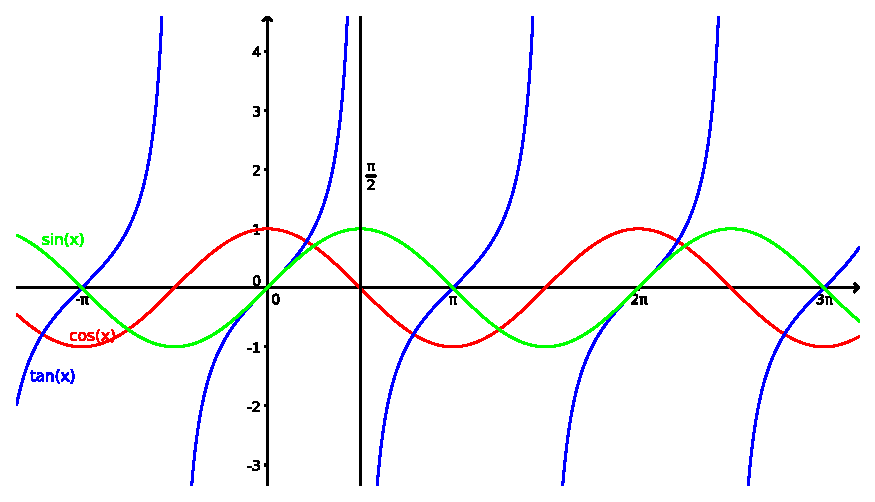
\includegraphics[width=\columnwidth]{sin_cos_tan.eps}

\subsubsection{Einheitskreis}
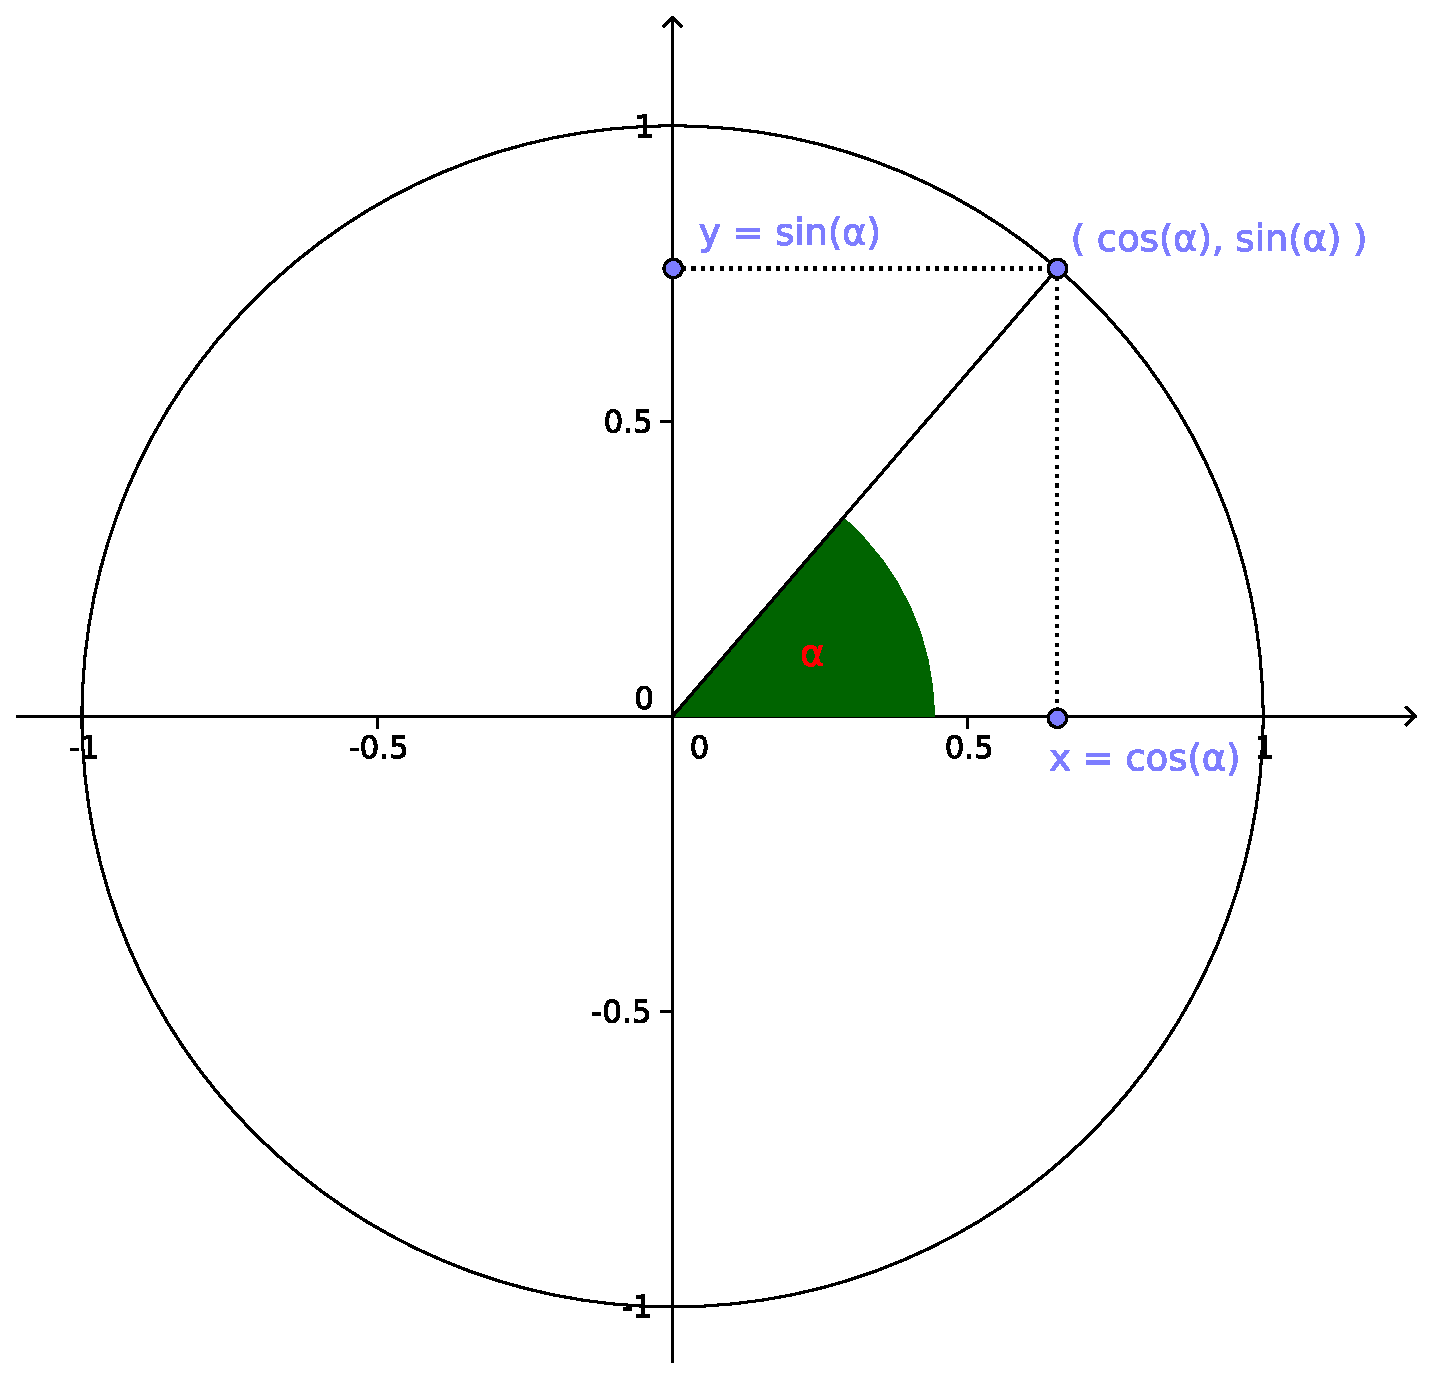
\includegraphics[width=\columnwidth]{einheitskreis_sin_cos.eps}
$\tan \alpha = \frac{\sin \alpha}{\cos \alpha} = \frac{y}{x}$

\subsection{Trigonometrische Funktionen \& Additionstheorem}
\begin{itemize}[leftmargin=*]
	\item $\sin^2(x) + \cos^2(x) = 1$
	\item $\frac{1}{\cos^2(\alpha)} = 1 + \tan^2(\alpha)$
	\item $\sin(90^\circ \pm \alpha) = \cos(\alpha)$
	\item $\sin(180^\circ \pm \alpha) = \mp \sin(\alpha)$
	\item $\cos(90^\circ \pm \alpha) = \mp \sin(\alpha)$
	\item $\cos(180^\circ \pm \alpha) = - \cos(\alpha)$
	\item $\sin(\alpha \pm \beta) = \sin(\alpha)\cos(\beta) \pm
	\cos(\alpha)\sin(\beta)$
	\item $\cos(\alpha \pm \beta) = \cos(\alpha)\cos(\beta) \mp \sin(\alpha)
	\sin(\beta)$
	\item $\tan(\alpha \pm \beta) = \frac{\tan(\alpha) \pm \tan(\beta)}{1 \mp
	\tan(\alpha)\tan(\beta)}$
	\item $\sin(2\alpha) = 2 \sin(\alpha)\cos(\alpha)$
	\item $\cos(2\alpha) = \cos^2(\alpha) - \sin^2(\alpha) = 2 \cos^2(\alpha) - 1
	= 1 - 2 \sin^2(\alpha)$
	\item $\tan(2\alpha) = \frac{2 \tan(\alpha)}{1 - \tan^2(\alpha)}$
\end{itemize}

\subsection{Hyperbelfunktionen}
\begin{itemize}[leftmargin=*]
	\item $\sinh(x) = \frac{1}{2}(e^x - e^{-x}) = -i \sin(ix)$
	\item $\cosh(x) = \frac{1}{2}(e^x + e^{-x}) = \cos(ix)$
	\item $\tanh(x) = \frac{\sinh(x)}{\cosh(x)} = \frac{e^x - e^{-x}}{e^x +
	e^{-x}} = \frac{e^{2x} - 1}{e^{2x} + 1} = 1 - \frac{2}{e^{2x} + 1}$
	\item $\arcsinh(x) = \ln(x + \sqrt{x^2 + 1})$
	\item $\arcosh(x) = \ln(x + \sqrt{x^2 - 1})$
	\item $\arctanh(x) = \frac{1}{2} \ln(\frac{1+x}{1-x})$
	\item Umformung: $\tanh(x) + 1 = \frac{e^{2x} - 1}{e^{2x} + 1} + 1 = \frac{2x -
	1 + e^{2x} + 1}{e^{2x} + 1} = \frac{2e^{2x}}{e^{2x} + 1}$
\end{itemize}


\subsection{Ableitungen}
\subsection{Regeln}
\begin{itemize}[leftmargin=*]
	\item (Summenregel) $(f + g)'(x) = f'(x) + g'(x)$
	\item (Produktregel) $(fg)'(x) = f'(x)g(x) + f(x)g'(x)$
	\item (Quotientenregel) $(\frac{f}{g})'(x) = \frac{f'(x)g(x) -
	f(x)g'(x)}{g^2(x)}$
	\item (Kettenregel) $(g \circ f)'(x) = (g(f(x)))' = g'(f(x)) f'(x)$
\end{itemize}

\subsection{Ableitungs-Tafel}
\begin{itemize}[leftmargin=*]
	\item $\frac{d}{dx}\; x^n = nx^{n-1}$
	\item $\frac{d}{dx}\; \frac{1}{x^n} = -n \frac{1}{x^{n+1}}$
	\item $\frac{d}{dx}\; \sqrt[n]{x} = \frac{1}{n\sqrt[n]{x^{n-1}}}$
	\item $\frac{d}{dx}\; e^{\alpha x + \beta} = \alpha e^{\alpha x + \beta}$
	\item $\frac{d}{dx}\; \ln(x) = \frac{1}{x}$
	\item $\frac{d}{dx}\; \alpha^x = \alpha^x \ln(\alpha)$
	\item $\frac{d}{dx}\; x^x = x^x (1 + \ln(x))$
	\item $\frac{d}{dx}\; \sin(\alpha x + \beta) = \alpha \cos(\alpha x + \beta)$
	\item $\frac{d}{dx}\; \cos(\alpha x + \beta) = -\alpha \sin(\alpha x + \beta)$
	\item $\frac{d}{dx}\; \tan(\alpha x + \beta) = \alpha \frac{1}{\cos^2(\alpha x
	+ \beta)}$
	\item $\frac{d}{dx}\; \sinh(\alpha x + \beta) = \alpha \cosh(\alpha x + \beta)$
	\item $\frac{d}{dx}\; \cosh(\alpha x + \beta) = \alpha \sinh(\alpha x + \beta)$
	\item $\frac{d}{dx}\; \tanh(\alpha x + \beta) = \alpha
	\frac{1}{\cosh^2(\alpha x + \beta)}$
	\item $\frac{d}{dx}\; \arcsin(\alpha x + \beta) =
	\frac{\alpha}{\sqrt{1-(\alpha x + \beta)^2}}$;  
		$\frac{d}{dx}\; \arcsin(x) = \frac{1}{\sqrt{1-x^2}}$
	\item $\frac{d}{dx}\; \arccos(\alpha x + \beta) = -\frac{\alpha}{\sqrt{1 -
	(\alpha x + \beta)^2}}$;
		$\frac{d}{dx}\; \arccos(x) = -\frac{1}{\sqrt{1-x^2}}$
	\item $\frac{d}{dx}\; \arctan(\alpha x + \beta) = \frac{\alpha}{(\alpha x +
	\beta)^2 + 1}$; 
		$\frac{d}{dx}\; \arctan(x) = \frac{1}{x^2+1}$
	\item $\frac{d}{dx}\; x^{x^\alpha} = x^{x^\alpha + \alpha - 1} (\alpha
	\log(x) + 1)$
	\item $\frac{d}{dx}\; e^{x^\alpha} = \alpha x^{\alpha - 1} e^{x^\alpha}$
\end{itemize}

\subsection{Integrale}
\subsubsection{Integralregeln}
Es gelte: $\int f(x) \, dx = F(x)$
\begin{itemize}[leftmargin=*]
	\item $\int u'\cdot v dx = uv - \int u \cdot v' dx$
	\item $\int f(x) dx = \int f(g(t)) \cdot g'(t) dt, \; x=g(t), dx = g'(t) dt$\newline\hfill
	\item $\int f(a + x) \,dx = F(a + x)$
	\item $\int f(a - x) \,dx = -F(a-x)$
	\item $\int f(-x) \,dx = -F(-x)$
	\item $\int f(\alpha x) \,dx = \frac{1}{\alpha}F(\alpha x)$
	\item $\int \frac{g'(x)}{g(x)} \, dx = \ln|g(x)|$
	\item $\int g(x)g'(x) \, dx = \frac{1}{2}g(x)^2$
\end{itemize}
\subsubsection{typische Integrale}
\begin{itemize}[leftmargin=*]
  	\item $\int \frac{1}{x} \,dx = \ln |x|$
  	\item $\int \frac{1}{x+a} \,dx = \ln |x+a|$
  	\item $\int \ln(x) \,dx = x(\ln(x) - 1)$
  	\item $\int \ln(ax + b) \,dx = \frac{(a x+b) \ln (a x+b)-a x}{a}$
  	\item $\int \frac{1}{(x+a)^2} \,dx = - \frac{1}{x+a}$
  	\item $\int \frac{1}{\sqrt{x}} \,dx = 2 \sqrt{x}$
	\item $\int \frac{1}{ax+b} \,dx = \frac{1}{a} \ln |ax+b|$
	\item $\int(ax + b)^n \,dx = \frac{(ax + b)^{n+1}}{(n + 1)a}, (n \neq -1)$
	\item $\int x(ax+b)^n \,dx = \frac{(ax + b)^{n+2}}{(n+2)a^2} -
	\frac{b(ax+b)^{n+1}}{(n+1)a^2}$
	\item $\int \frac{ax + b}{px + q} \,dx = \frac{ax}{p} + \frac{bp - aq}{p^2} \ln
	|pq+q|$
	\item $\int \frac{1}{a^2 + x^2} \,dx = \frac{1}{a} \arctan(\frac{x}{a})$
	\item $\int \frac{1}{a^2 - x^2} \,dx = \frac{1}{2a} \ln \left | \frac{a+x}{a-x}
	\right |$
	\item $\int \sqrt{x} \,dx = \frac{2}{3}\sqrt{x^3}$
	\item $\int a^{xb + c} \,dx = \frac{a^{bx + c}}{b \log(a)}$
\end{itemize}

\subsubsection{trionometrische Funktionen}
\begin{itemize}[leftmargin=*]
	\item $\int \sin(ax) \,dx = -\frac{1}{a}\cos(ax)$
	\item $\int \cos(ax) \,dx = \frac{1}{a}\sin(ax)$
	\item $\int \sin(ax)^2 \,dx = \frac{x}{2} - \frac{sin(2ax)}{4a}$
	\item $\int \frac{1}{\sin^2 x} \,dx = -\cot x$
	\item $\int x \sin(ax) \,dx = \frac{\sin(ax)}{a^2} - \frac{x \cos(ax)}{a}$
	\item $\int \cos^2(ax) \,dx = \frac{x}{2} + \frac{\sin(2ax)}{4a}$
	\item $\int \frac{1}{\cos^2(x)} \,dx = \tan x$
	\item $\int \cos(ax) \,dx = \frac{\cos(ax)}{a^2} + \frac{x \sin(ax)}{a}$
	\item $\int \sin(ax) \cos(ax) \,dx = -\frac{\cos^2(ax)}{2a}$
	\item $\int \tan(ax) \,dx = - \frac{1}{a} \ln | \cos(ax) |$
	\item $\int \arcsin(x) \,dx = x \arcsin(x) + \sqrt{1 - x^2}$
	\item $\int \arccos(x) \,dx = x \arccos(x) - \sqrt(1-x^2)$
	\item $\int \arctan(x) \,dx = x \arctan(x) - \frac{1}{2} \ln(1+x^2)$
\end{itemize}

\subsubsection{Hyperbelfunktionen}
\begin{itemize}[leftmargin=*]
	\item $\int \sinh(ax + b) \,dx = \frac{\cosh(ax + b)}{a}$; $\int \sinh(x) \,dx
	= \cosh(x)$
	\item $\int \cosh(ax + b) \,dx = \frac{\sinh(ax + b)}{a}$; $\int \cosh(x) \,dx
	= \sinh(x)$
	\item $\int \tan(ax + b) \,dx = \frac{\log(\cosh(ax+b))}{a}$; $\int \tan(x)
	\,dx = \log(\cosh(x))$
\end{itemize}

\subsubsection{Exponentialfunktion}
\begin{itemize}[leftmargin=*]
  	\item $\int e^{ax} \,dx = \frac{1}{a} e^{ax}$ 
	\item $\int x e^{ax} \,dx = e^{ax} \cdot \left ( \frac{ax - 1}{a^2} \right )$
	\item $\int x \ln(x) \,dx = \frac{1}{2} x^2 (\ln(x) - \frac{1}{2})$
	\item $\int_{-\infty}^\infty e^{-\frac{1}{a}x^2} \,dx = \sqrt{a \pi}$
\end{itemize}

\subsection{Reihenentwicklung}
\begin{itemize}[leftmargin=*]
	\item $e^x = \sum_{n=0}^\infty \frac{x^n}{n!} = 1 + \frac{x}{1!} +
	\frac{x^2}{2!} + \cdots$
	\item $\sin x = \sum_{n=0}^\infty (-1)^n \frac{x^{2n + 1}}{(2n + 1)!} = x -
	\frac{x^3}{3!} + \frac{x^2}{5!} + \cdots$
	\item $\cos x = \sum_{n=0}^\infty (-1)^n \frac{x^{2n}}{(2n)!} = 1 -
	\frac{x^2}{2!} + \frac{x^4}{4!} - \cdots + \cdots$
	\item $\sinh x = \sum_{n=0}^\infty \frac{x^{2n+1}}{(2n + 1)!}$
	\item $\cosh x = \sum_{n=0}^\infty \frac{x^{2n}}{(2n)!}$
	\item $\ln x = \sum_{n=0}^\infty \frac{2}{2n + 1} \cdot \left(
	\frac{x-1}{x+1} \right)^{2n}$
\end{itemize}

\subsection{Grenzwerte}
\begin{itemize}[leftmargin=*]
	\item \textbf{Bernoullische Ungleichung}: $x \geq -1, n \in \N: \; (1+x)^n \geq
	1+nx$
	\item \textbf{Vergleich von Folgen}: weiter rechts stehende Folgen streben
	schneller gegen $\infty$ als die links davon stehenden: $1, \quad \ln n, \quad
	n^\alpha (\alpha > 0), \quad q^n (q > 1), \quad n!, \quad n^n$ $\Rightarrow
	\lim_{x \to \infty} \frac{\ln n}{n^\alpha} = 0$
\end{itemize}
\subsubsection{$\lim_{n \to \infty}$}
\begin{itemize}[leftmargin=*]
	\item $\lim_{n \to \infty} \sqrt[n]{a} \rightarrow 1$
	\item $\lim_{n \to \infty} \sqrt[n]{n} \rightarrow 1$
	\item $\lim_{n \to \infty} \sqrt[n]{n!} \rightarrow \infty$
	\item $\lim_{n \to \infty} \frac{n}{\sqrt[n]{n!}} \rightarrow e$
	\item $\lim_{n \to \infty} \frac{1}{n} \sqrt[n]{n!} \rightarrow \frac{1}{e}$
	\item $\lim_{n \to \infty} \left ( \frac{n+1}{n} \right )^n \rightarrow e$
	\item $\lim_{n \to \infty} \left ( 1 + \frac{1}{n} \right )^n \rightarrow e$
	\item $\lim_{n \to \infty} \left ( 1 - \frac{1}{n} \right )^n \rightarrow \frac{1}{e}$
	\item $\lim_{n \to \infty} \left ( 1 + \frac{x}{n} \right )^n \rightarrow e^x$
	\item $\lim_{n \to \infty} \left ( 1 - \frac{x}{n} \right )^n \rightarrow \frac{1}{e^x}$
	\item $\lim_{n \to \infty} {a \choose n} \rightarrow 0, \; a > -1$
	\item $\lim_{n \to \infty} \frac{a^n}{n!} \rightarrow 0$
	\item $\lim_{n \to \infty} \frac{n^n}{n!} \rightarrow \infty$
	\item $\lim_{n \to \infty} \frac{a^n}{n^k} \rightarrow \infty, a > 1, k$ fest
	\item $\lim_{n \to \infty} a^n n^k \rightarrow 0, |a| < 1, k$ fest
	\item $\lim_{n \to \infty} n(\sqrt[n]{a} - 1) \rightarrow \ln a, a > 0$
	\item $\lim_{n \to \infty} \left( 1+\frac{x}{n} \right)^n = e^x \quad$
	\item $\lim_{n \to \infty} \sqrt[n]{n} = 1$
	\item $\lim_{n \to \infty} n^p q^n = 0 \qquad p \in \N \text{ und } 0 < q < 1$
	\item $\lim_{x \to \infty} \sqrt{x^2-x}-x = \frac{1}{2}$ \newline{\small (Lösungsansatz mit Taylorreihe
	($\sqrt{1-x} = 1 + \frac{x}{2}+O(x^2)$): $\sqrt{x^2-x}-x = x(\sqrt{1-\frac{1}{x}}-1) =
	x((1+\frac{1}{2x}+O(\frac{1}{x^2}))-1) = \frac{1}{2}+O(\frac{1}{x}) \underset{n \to \infty}{\longrightarrow} \frac{1}{2}$ )}
\end{itemize}
\subsubsection{$\lim_{x \to 0}$}
\begin{itemize}[leftmargin=*]
	\item $\lim_{x \to 0} \frac{a^x - 1}{x} = \ln a$
	\item $\lim_{x \to 0} \frac{\sin x}{x} = 1$
	\item $\lim_{x \to 0} \frac{1 - \cos x}{x} = 0$
	\item $\lim_{x \to 0} \frac{\log_a (1 + x)}{x} = \frac{1}{\ln a}$
	\item $\lim_{x \to 0} x^a \ln x = 0, \; a  > 0$
	\item $\lim_{x \to 0} \frac{a^x-1}{x} = \ln a$ 
	\item $\lim_{x \to 0} \frac{\sin(x)}{x} = 1$ 
	\item $\lim_{x \to 0} \frac{1-\cos(x)}{x} = 0 \quad$ 
	\item $\lim_{x \to 0} \frac{\log_a(1+x)}{x} = \frac{1}{\ln a}$
	\item $\lim_{x \to 0} x^\alpha \ln x = 0 \qquad \alpha > 0$
\end{itemize}

\subsection{Reihen}
\begin{itemize}[leftmargin=*]
	\item $\sum_{n=1}^\infty \frac{1}{n}$ divergiert (``harmonische Reihe'')
	\item $\sum_{n=1}^\infty \frac{(-1)^n}{n} = \ln \frac{1}{2}$
	\item $\sum_{n=1}^\infty \frac{1}{n^\alpha}$ konvergiert für $\alpha > 1$,
	divergiert für $\alpha \leq 1$
	\item $\sum_{n=1}^m n = \frac{m(m+1)}{2}$
	\item $\sum_{n=0}^\infty q^n = \frac{1}{1-q}$ für $|q| < 1$ (``geometrische
	Reihe'')
	\item $\sum_{n=0}^\infty (-1)^n q^n = \frac{1}{1-q}$ für $|q| < 1$ (``geometrische
	Reihe'')
	\item $\sum_{n=1}^\infty \frac{1}{n^2} = \frac{\pi^2}{6}$
	\item $\sum_{n=0}^m q^n = \frac{1-q^{m+1}}{1-q}$ 
	% ist in einer serie vorgekommen:
	\item  $\sum_{n=0}^m n^2 = \frac{1}{6}m(m+1)(2m+1)$
	\item  $\sum_{n=0}^m n^3 = \frac{1}{4}m^2(m+1)^2$
\end{itemize}

\subsection{Kreuzprodukt}
{\footnotesize
\[
\vec{a} \times \vec{b} = \left ( \begin{array}{c} a_1 \\ a_2 \\ a_3 \end{array}
\right ) \times
\left ( \begin{array}{c} b_1 \\ b_2 \\ b_3 \end{array}
\right ) =
\left ( \begin{array}{c} a_2b_3 - a_3b_2 \\ a_3b_1 - a_1b_3 \\ a_1b_2 - a_2b_1
\end{array} \right )
\]
}

\begin{multicols}{2}
\subsection{Exponent}
\begin{itemize}[leftmargin=*]
  \item $a^n a^m = a^{n + m}$
  \item $(a^n)^m = a^{nm}$
  \item $(ab)^n = a^n b^n$
  \item $\left( \frac{a}{b} \right)^n = \frac{a^n}{b^n}$
  \item $a^{-n} = \frac{1}{a^n}$
  \item $\left( \frac{a}{b} \right)^{-n} = \left( \frac{b}{a} \right)^n$
  \item $a^\frac{n}{m} = (a^\frac{1}{m})^n = (a^n)^\frac{1}{m}$
\end{itemize}
\columnbreak

\subsection{Wurzel}
\begin{itemize}[leftmargin=*]
  \item $\sqrt[n]{a} = a^\frac{1}{n}$
  \item $\sqrt[n]{ab} = \sqrt[n]{a} \sqrt[n]{b}$
  \item $\sqrt[m]{\sqrt[n]{a}} = \sqrt[nm]{a}$
  \item $\sqrt[n]{\frac{a}{b}} = \frac{\sqrt[n]{a}}{\sqrt[n]{b}}$
\end{itemize}

\end{multicols}

\subsection{Ungleichungen}
\begin{itemize}[leftmargin=*]
  \item $a < b \Rightarrow a + c < b + c$ und $a - c < b - c$
  \item $a < b$ und $c > 0 \Rightarrow \frac{a}{c} < \frac{b}{c}$
  \item $a < b$ und $c < 0 \Rightarrow \frac{a}{c} > \frac{b}{c}$ 
  \item Dreiecksungleichung für reelle Zahlen: $|a+b| \le |a|{+}|b|$ %Quelle Wikipedia: http://de.wikipedia.org/wiki/Dreiecksungleichung#Dreiecksungleichung_f.C3.BCr_reelle_Zahlen
  \item Cauchy-Schwarz Ungleichung: $|x \cdot y| \leq \|x\| \cdot \|y\|, \; x,y \in \R^n$
\end{itemize}

\subsection{Logarithmen}
\begin{itemize}[leftmargin=*]
  \item $y = \log_a x \Leftrightarrow x = a^y$
  \item $\log_a 1 = 0$
  \item $\log_a a^x = x$
  \item $a^{\log_a x} = x $
  \item $\log_a xy = \log_a x + \log_a y$
  \item $\log_a \frac{1}{x} = - \log_a x$
  \item $\log_a x^r = r \log_a x$
  \item $\log_a x = \frac{\log_b x}{\log_b a}$
  \item $\log_a x = \frac{\ln x}{\ln a}$
  \item $\log_a (x+y) = \log_a x + log_a (1 + \frac{y}{x})$
  \item $\log_a (x-y) = \log_a x + \log_a (1- \frac{y}{x})$
\end{itemize}

\subsection{Komplexe Zahlen}
\begin{itemize}[leftmargin=*]
	\item $z \in \C: z = a + b\cdot i$
	\item $i^2 = -1$
	\item $(a + bi) + (c + di) = (a + c) + (b + d)i$
	\item $(a + bi) \cdot (c + di) = (ac - bd) + (ad + bc)i$
	\item $\frac{a + bi}{c + di} = \frac{ac + bd}{c^2 + d^2} + \frac{bc - ad}{c^2 + d^2}\cdot i$
\end{itemize}

\subsection{Geometrische Körper}
\subsubsection{Ellipsoid}
Hat die Form eines Rugbyballs. In kartesischen Koordinaten definert durch
$\frac{x^2}{a^2} + \frac{y^2}{b^2} + \frac{z^2}{c^2} - 1 = 0$.

\subsection{Ausklammern}
\begin{itemize}[leftmargin=*]
	\item $x^n - y^n = (x-y) (x^{n-1} + x^{n-2}y + x^{n-3}y^2 + \ldots + xy^{n-2}
	+ y^{n-1})$
	\item $x^n - 1 = (x-1)(x^{n-1} + x^{n-2} + \ldots + x + 1)$
\end{itemize}

\subsection{Aus Serien}
\begin{itemize}[leftmargin=*]
	\item Ableitung von $x^x$ kann man berechnen, indem man $x = e^{\log(x)}$
	setzt. Also in diesem Fall $e^{\log(x^x)} = e^{x \log(x)}$ ableitet, was $e^{x
	\log(x)} (1 + \log(x))$ (Serie 10)
	\item Cauchy-Schwarz Ungleichung: $|x \cdot y| \leq \|x\| \cdot \|y\|, \; x,y \in \R^n$
	\item Euler Identität (komplexe Zahlen): $e^{ix} = \cos(x) + i \sin(x)$
\end{itemize}

\begin{landscape}\begin{multicols}{3}

\subsection{\texorpdfstring{$\log(x)$}{log(x)}}
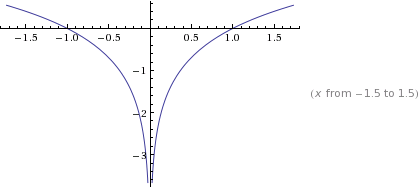
\includegraphics[scale=0.5]{log_x.png}

\subsection{\texorpdfstring{$\frac{1}{x}$}{1/x}}
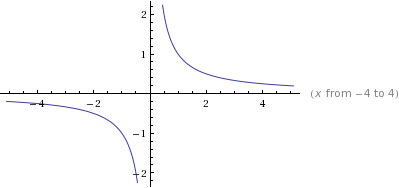
\includegraphics[scale=0.5]{1_over_x.png}

\subsection{\texorpdfstring{$\sqrt{x}$}{x^(1/x)}}
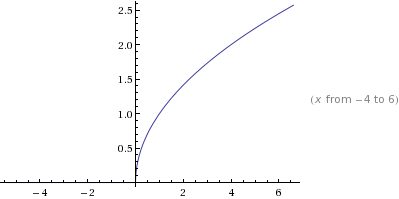
\includegraphics[scale=0.5]{sqrt_x.png}

\subsection{Funktionsmanipulation}
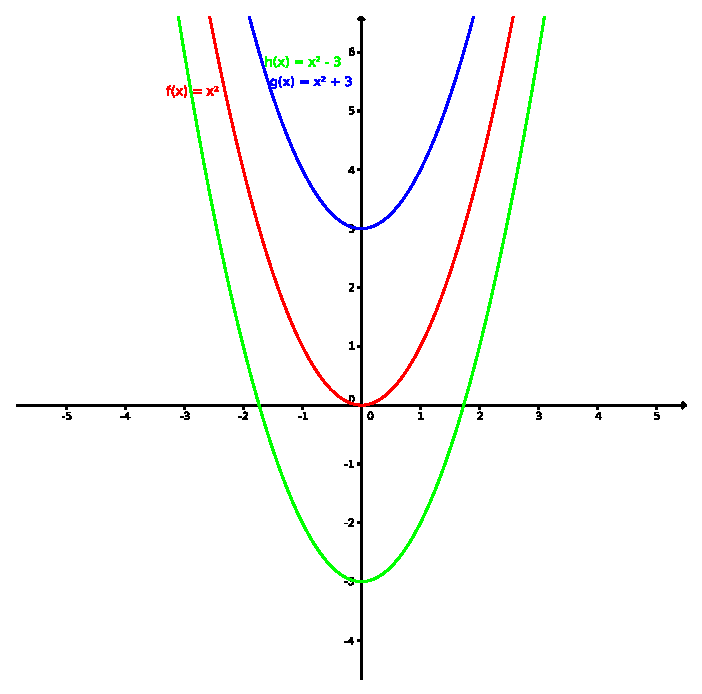
\includegraphics[width=\columnwidth]{manipulation_1.eps}
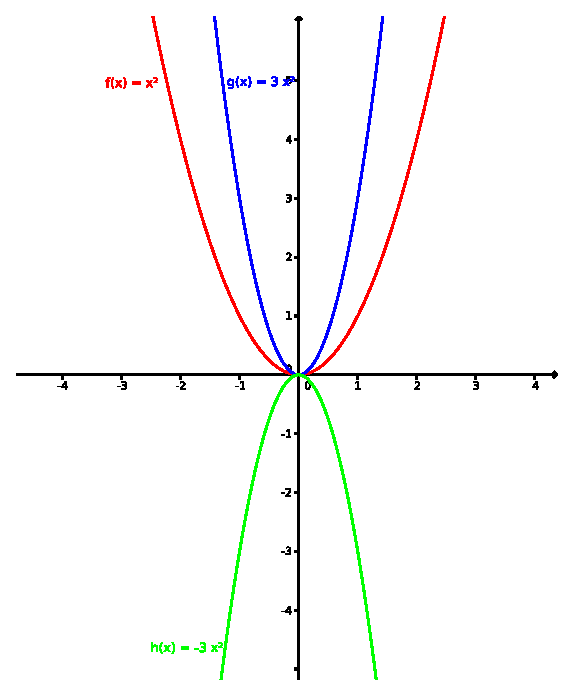
\includegraphics[width=\columnwidth]{manipulation_2.eps}
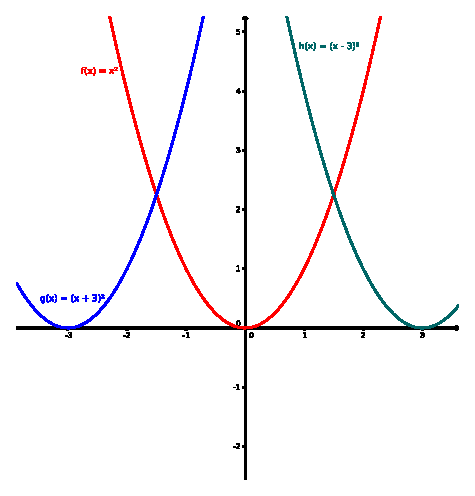
\includegraphics[width=\columnwidth]{manipulation_3.eps}

\subsection{Pascalsches Dreieck}
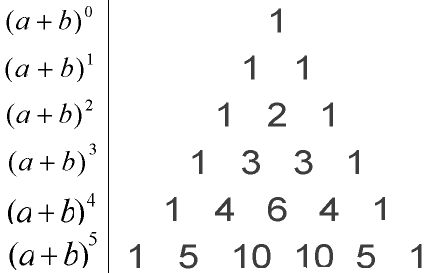
\includegraphics[width=\columnwidth]{pascal.png}

\end{multicols}\end{landscape}


% fill the page
\clearpage

\end{document}
